\documentclass[a4paper,12pt]{article}
\usepackage{amsmath,amssymb,amsfonts,amsthm}
\usepackage{tikz}
\usepackage [utf8x] {inputenc}
\usepackage [T2A] {fontenc} 
\usepackage[russian]{babel}
\usepackage{cmap} 

% Так ссылки в PDF будут активны
\usepackage[unicode]{hyperref}

% вы сможете вставлять картинки командой \includegraphics[width=0.7\textwidth]{ИМЯ ФАЙЛА}
% получается подключать, как минимум, файлы .pdf, .jpg, .png.
\usepackage{graphicx}
% Если вы хотите явно указать поля:
\usepackage[margin=1in]{geometry}
% Или если вы хотите задать поля менее явно (чем больше DIV, тем больше места под текст):
% \usepackage[DIV=10]{typearea}

\usepackage{fancyhdr}

\newcommand{\bbR}{\mathbb R}%теперь вместо длинной команды \mathbb R (множество вещественных чисел) можно писать короткую запись \bbR. Вместо \bbR вы можете вписать любую строчку букв, которая начинается с '\'.
\newcommand{\eps}{\varepsilon}
\newcommand{\bbN}{\mathbb N}
\newcommand{\dif}{\mathrm{d}}

\newtheorem{Def}{Определение}


\pagestyle{fancy}
\makeatletter % сделать "@" "буквой", а не "спецсимволом" - можно использовать "служебные" команды, содержащие @ в названии
\fancyhead[L]{\footnotesize Термодинамика и молекулярная физика}%Это будет написано вверху страницы слева
\fancyhead[R]{\footnotesize ФМХФ МФТИ}
\fancyfoot[L]{\footnotesize \@author}%имя автора будет написано внизу страницы слева
\fancyfoot[R]{\thepage}%номер страницы —- внизу справа
\fancyfoot[C]{}%по центру внизу страницы пусто

\renewcommand{\maketitle}{%
	\noindent{\bfseries\scshape\large\@title\ \mdseries\upshape}\par
	\noindent {\large\itshape\@author}
	\vskip 2ex}
\makeatother
\def\dd#1#2{\frac{\partial#1}{\partial#2}}


\title{2.1.3 \\ Определение $\frac{C_p}{C_v}$ по скорости звука в газе}
\author{Егор Берсенев} 
\date{15 марта 2016 г.}

\begin{document}
	\maketitle
	\section{Цель работы}
		\begin{enumerate}
			\item Измерение частоты колебаний и длины волны при резонансе звуковых колебаний в газе, заполняющем трубу.
			\item Определение показателя адиабаты с помощью уравнения состояния идеального газа.
		\end{enumerate}
	\section{Оборудование}
		Звуковой генератор ГЗ, электронный осциллограф, микрофон, телефон, раздвижная труба, теплоизолированная труба, термостат, баллон со сжатым углекислым газом, газгольдер.
	\section{Теоретическая часть}
		Скорость распространения звуковой волны в газах зависит от показателя адиабаты. На измерении скорости звука основан один из самых точных методово определения показателя адиабаты. Скорость звука в идеальном газе определяется формулой:
		\begin{equation}
			c = \sqrt{\gamma\frac{RT}{\mu}},
		\end{equation}
		где $R$ --- газовая постоянная, $T$ --- температура газа, $\mu$ --- молярная масса.
		Преобразуем:
		\begin{equation}
			\gamma=\frac{\mu}{RT}c^2
		\end{equation}.
		
		Звуковая волна, распространяющаяся вдоль трубы, испытывает многократные отражения, при этом наступает резонанс --- амплитуда резко возрастает.
		Скорость звука связана с его частотой $f$ и длиной волны $\lambda$ следующим соотношением:
		\begin{equation}
			c = \lambda f
		\end{equation}
		Подберем условия для резонанса двумя способами:
		\begin{enumerate}
			\item При неизменной частоте звукового генератора $L_n = n\frac{\lambda}{2}$. $\frac{\lambda}{2}$---угловой коэффициент $L(k)$.
			\item При постоянной длине трубы. $L = \frac{\lambda_1}{2}n = \frac{\lambda_2}{2}(n+1) \implies f_{k+1} = f_1+\frac{c}{2L}k$
		\end{enumerate}
		\section{Ход работы}
		\subsection{Измерения на неподвижной трубе}
		$L_{\text{тр}}=740\pm1\,\text{мм}$
		
		Проведем измерения резонансных частот на неподвижной трубе при разных температурах.
		\begin{center}
			\begin{tabular}{ l | l | l | l | l | l | l | l | l | l }
				\multicolumn{2}{c}{$T = 23.6$} & \multicolumn{2}{|c}{$T = 30.1$} & \multicolumn{2}{|c}{$T = 40$} & \multicolumn{2}{|c}{$T = 50$} & \multicolumn{2}{|c}{$T = 59$}\\ \hline
				n & $f$, Гц & n & $f$, Гц & n & $f$, Гц & n & $f$, Гц & n & $f$, Гц \\ \hline
				1 & 241.1 & 1 & 242 & 1 & 253 & 1 & 252  & 1 & 261 \\ \hline
				2 & 447.7 & 2 & 471.3 & 2 & 482.6 & 2 & 490 & 2 & 506  \\ \hline
				3 & 700.5 & 3 & 711.3 & 3 & 718.4 & 3 & 735 & 3 & 745  \\ \hline
				4 & 930 & 4 & 941 & 4 & 953.1 & 4 & 974 & 4 & 981  \\ \hline
				5 & 1162 & 5 & 1174 & 5 & 1194 & 5 & 1212 & 5 & 1226  \\ \hline
				6 & 1391 & 6 & 1407 & 6 & 1431 & 6 & 1456 & 6 & 1147  \\ \hline
			\end{tabular}
		\end{center}
		
		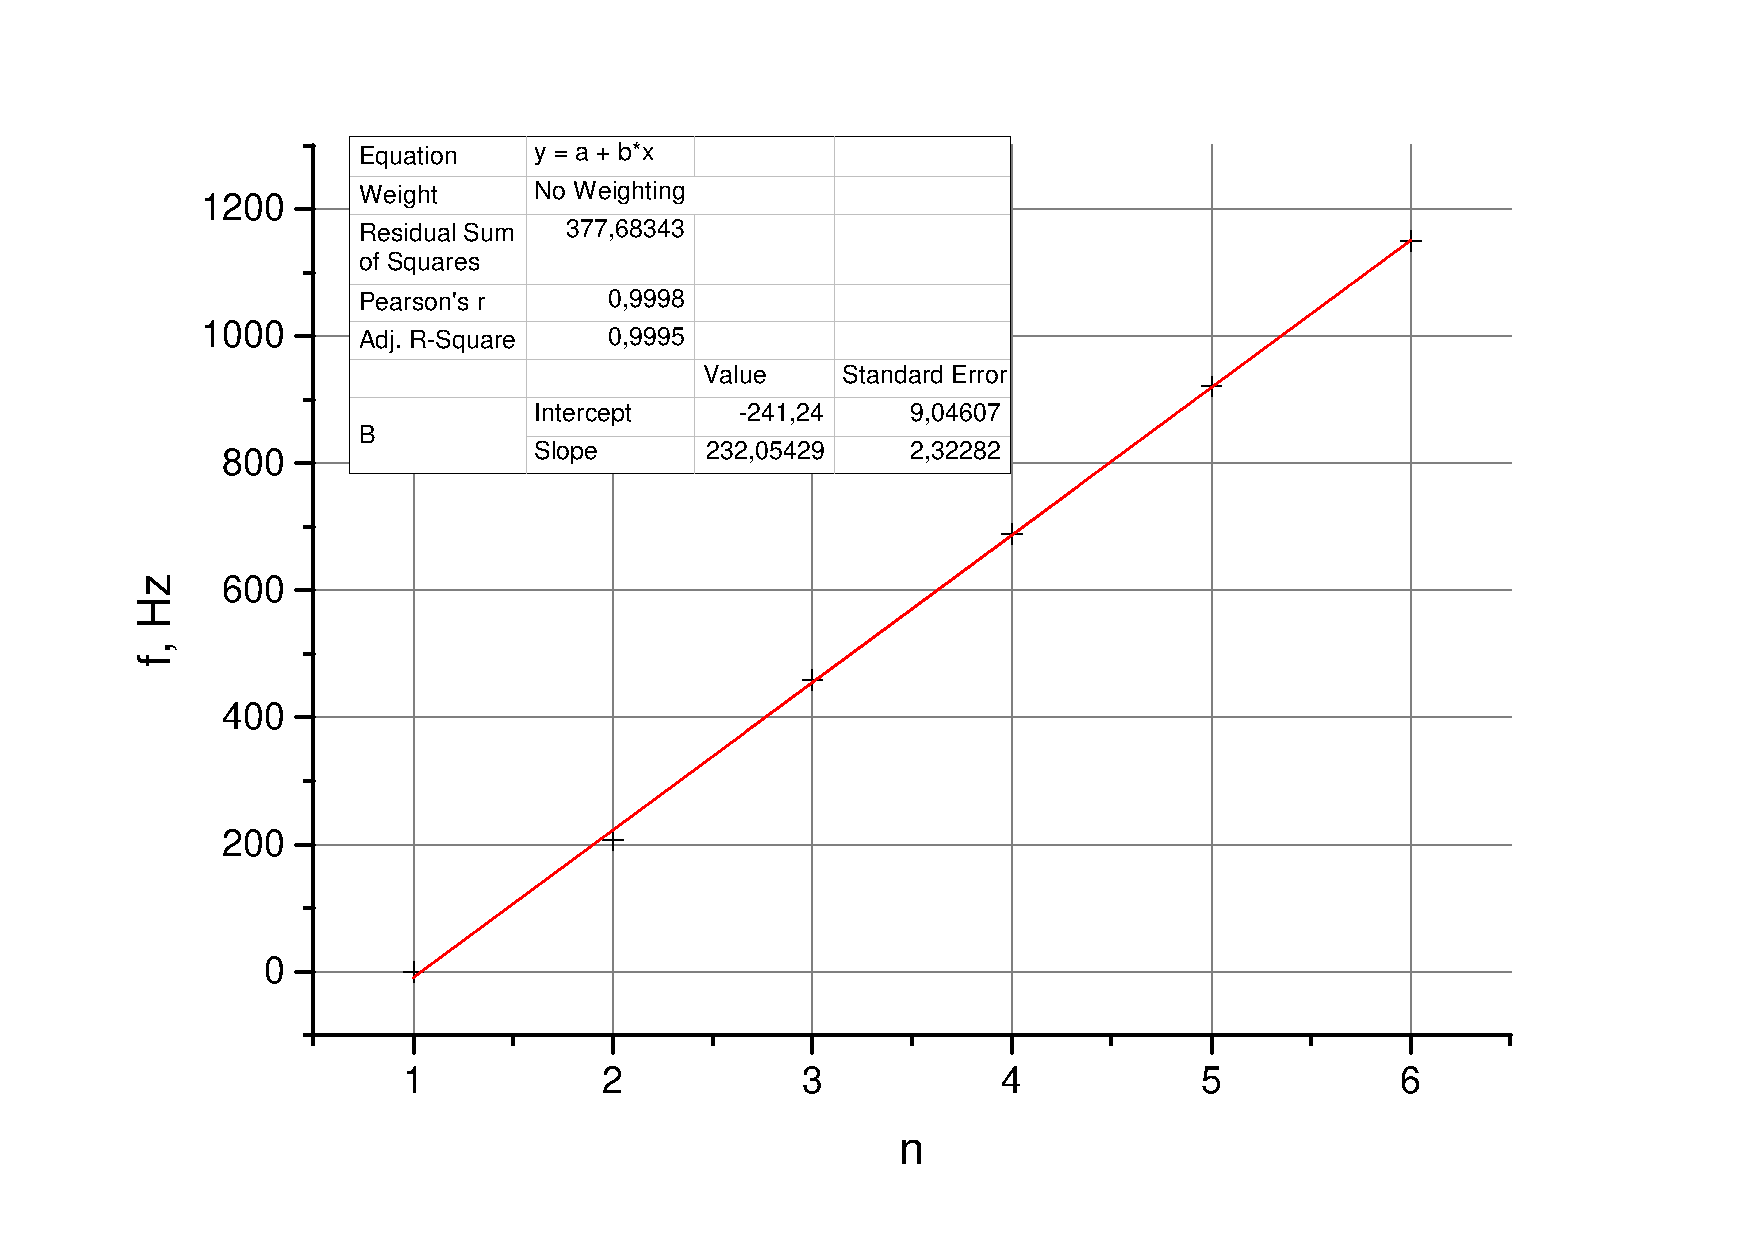
\includegraphics[width = 0.9\linewidth]{Graph1gr}
		
		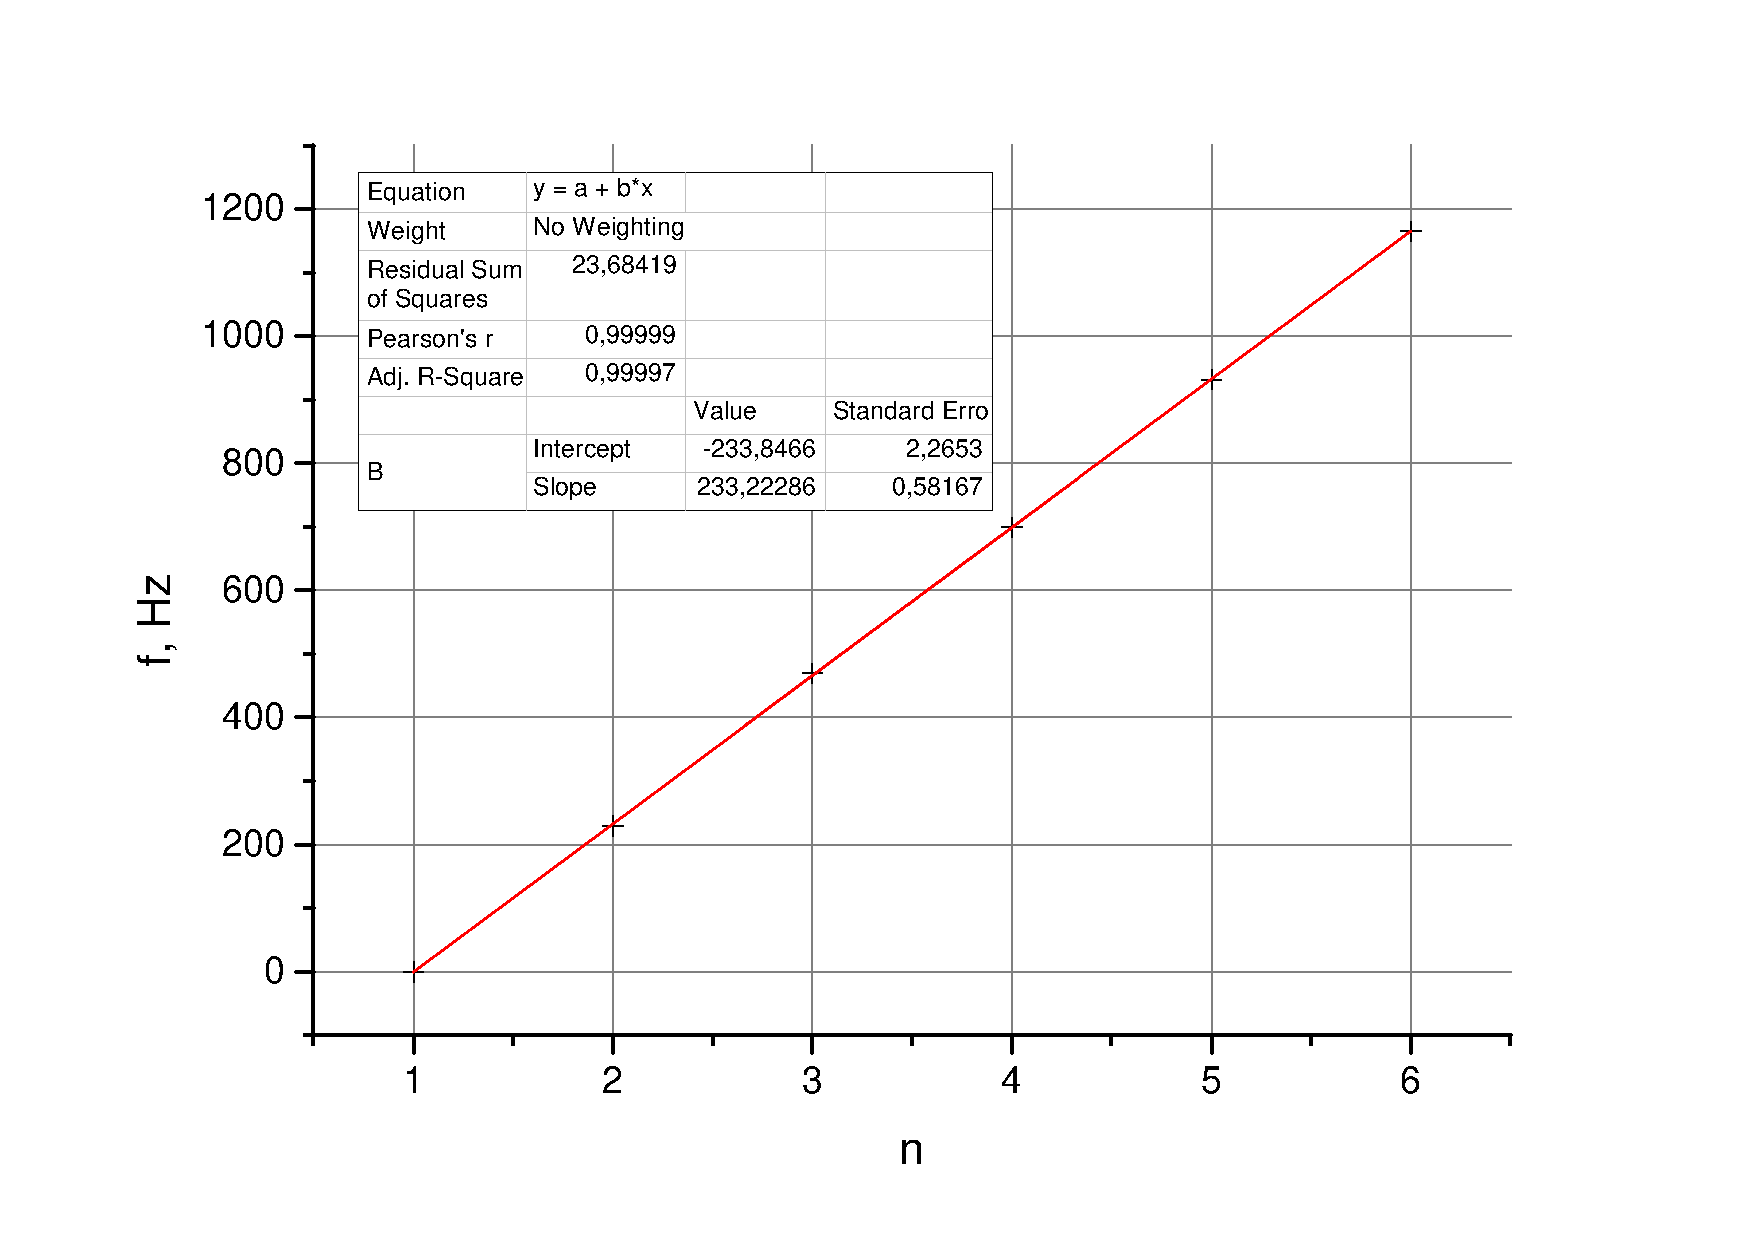
\includegraphics[width = 0.9\linewidth]{Graph2gr}
		
		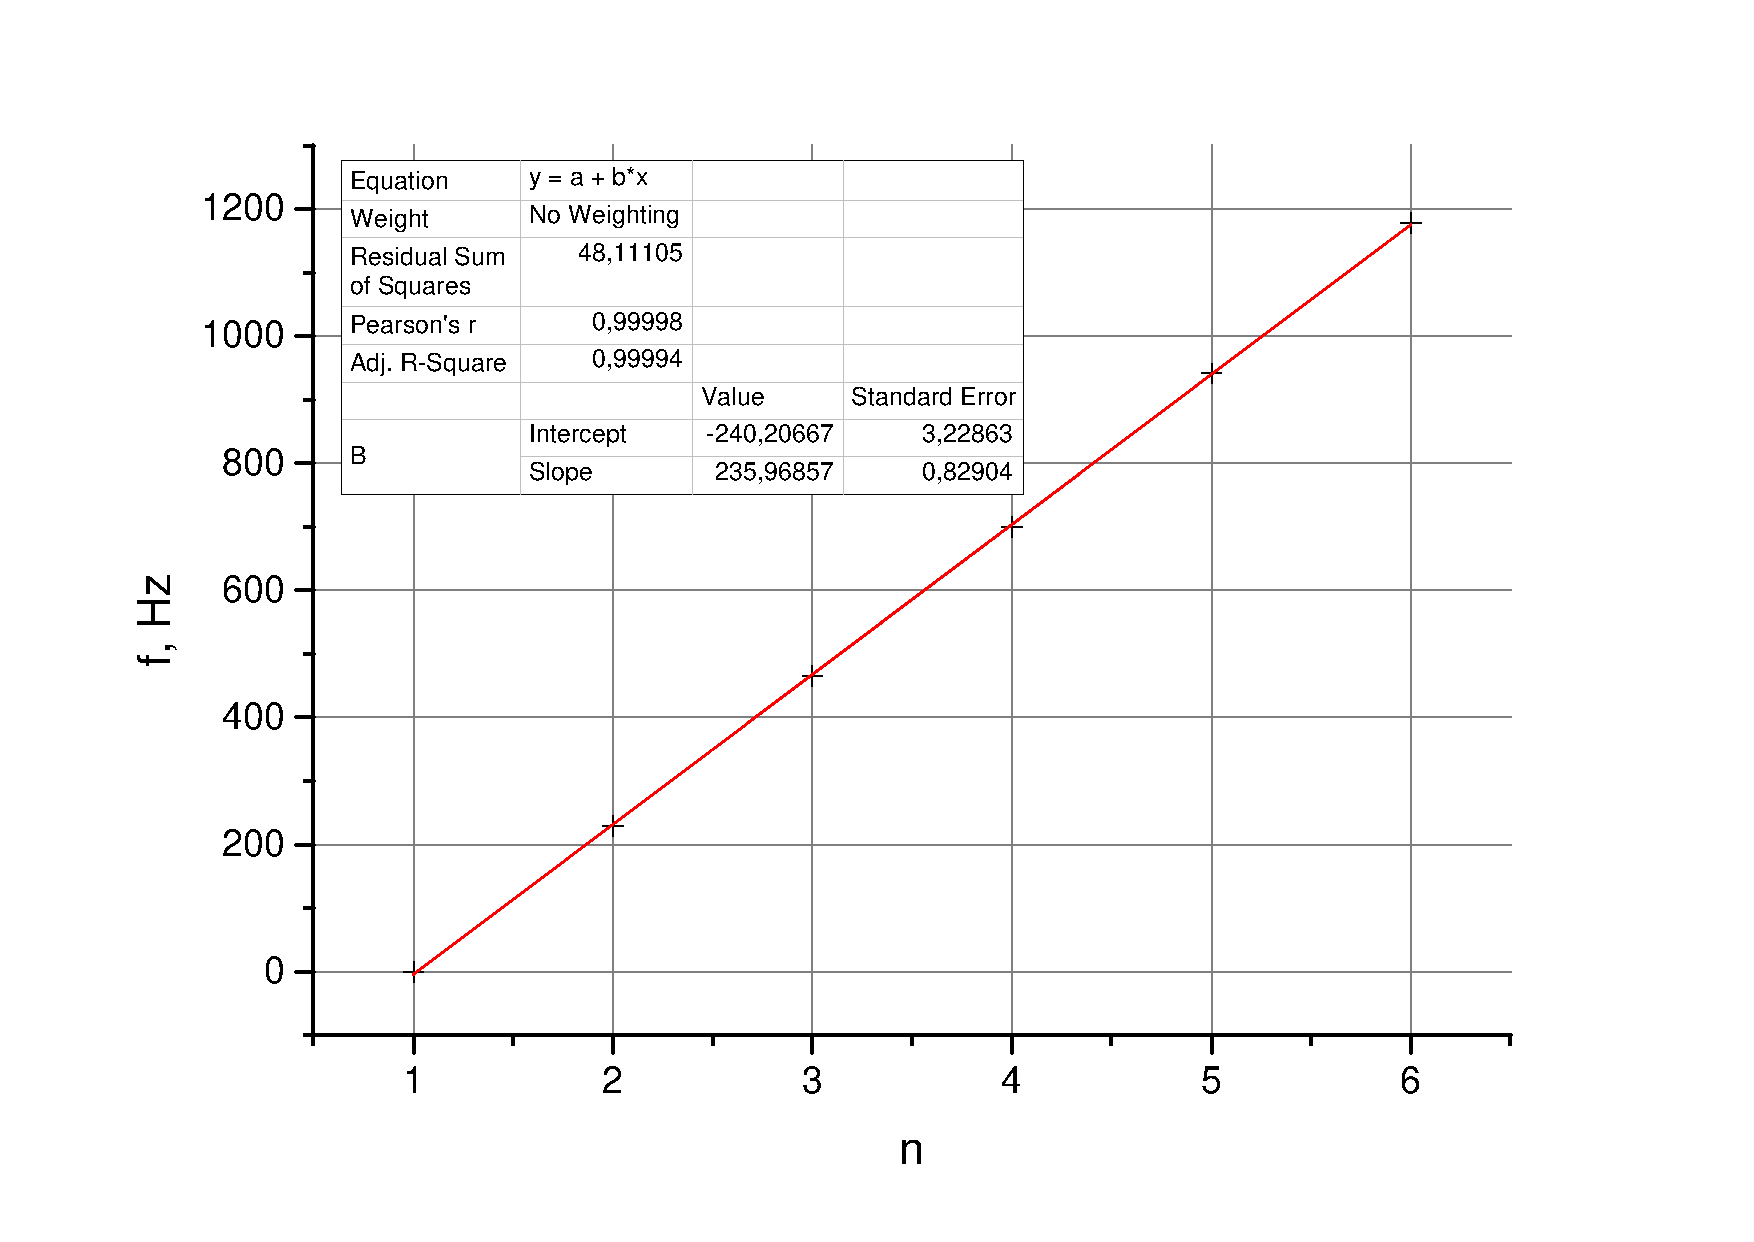
\includegraphics[width = 0.9\linewidth]{Graph3gr}
		
		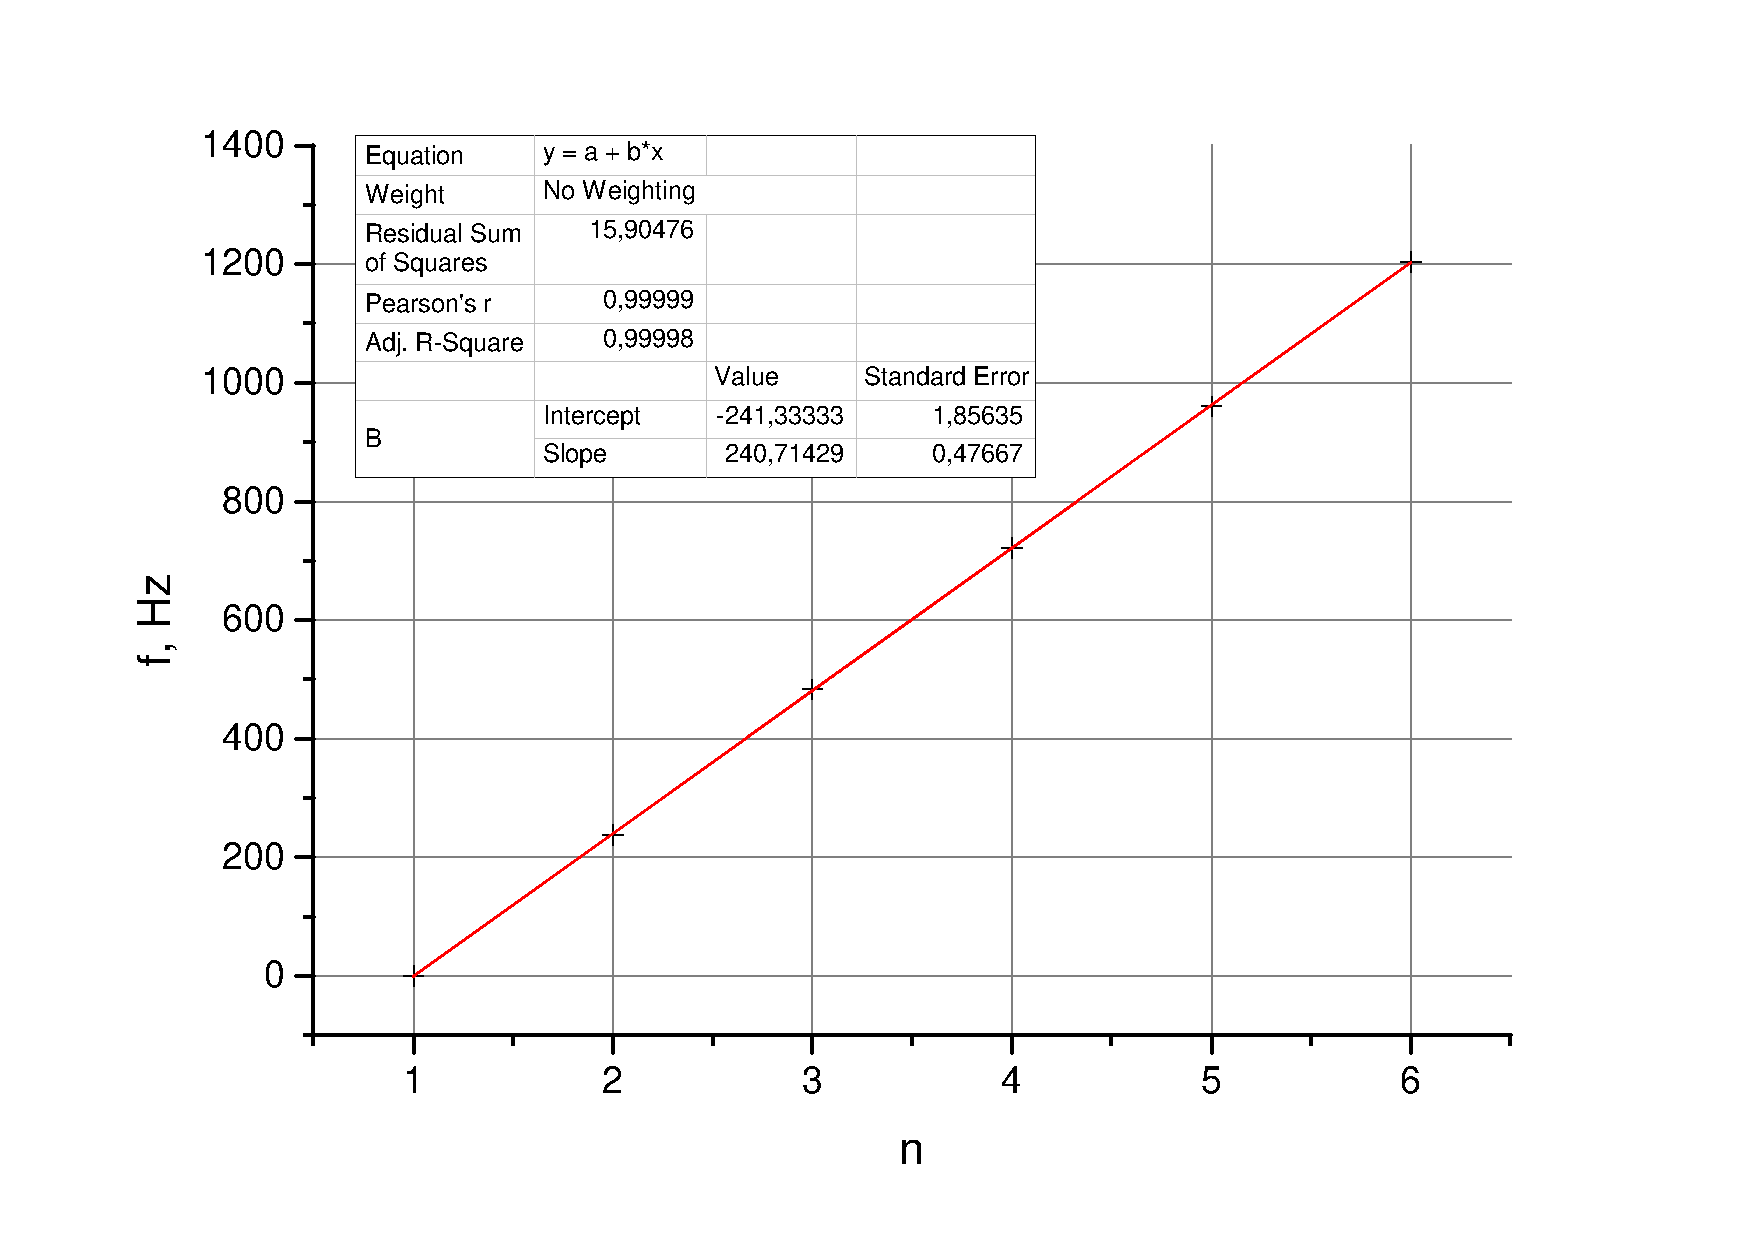
\includegraphics[width = 0.9\linewidth]{Graph4gr}
		
		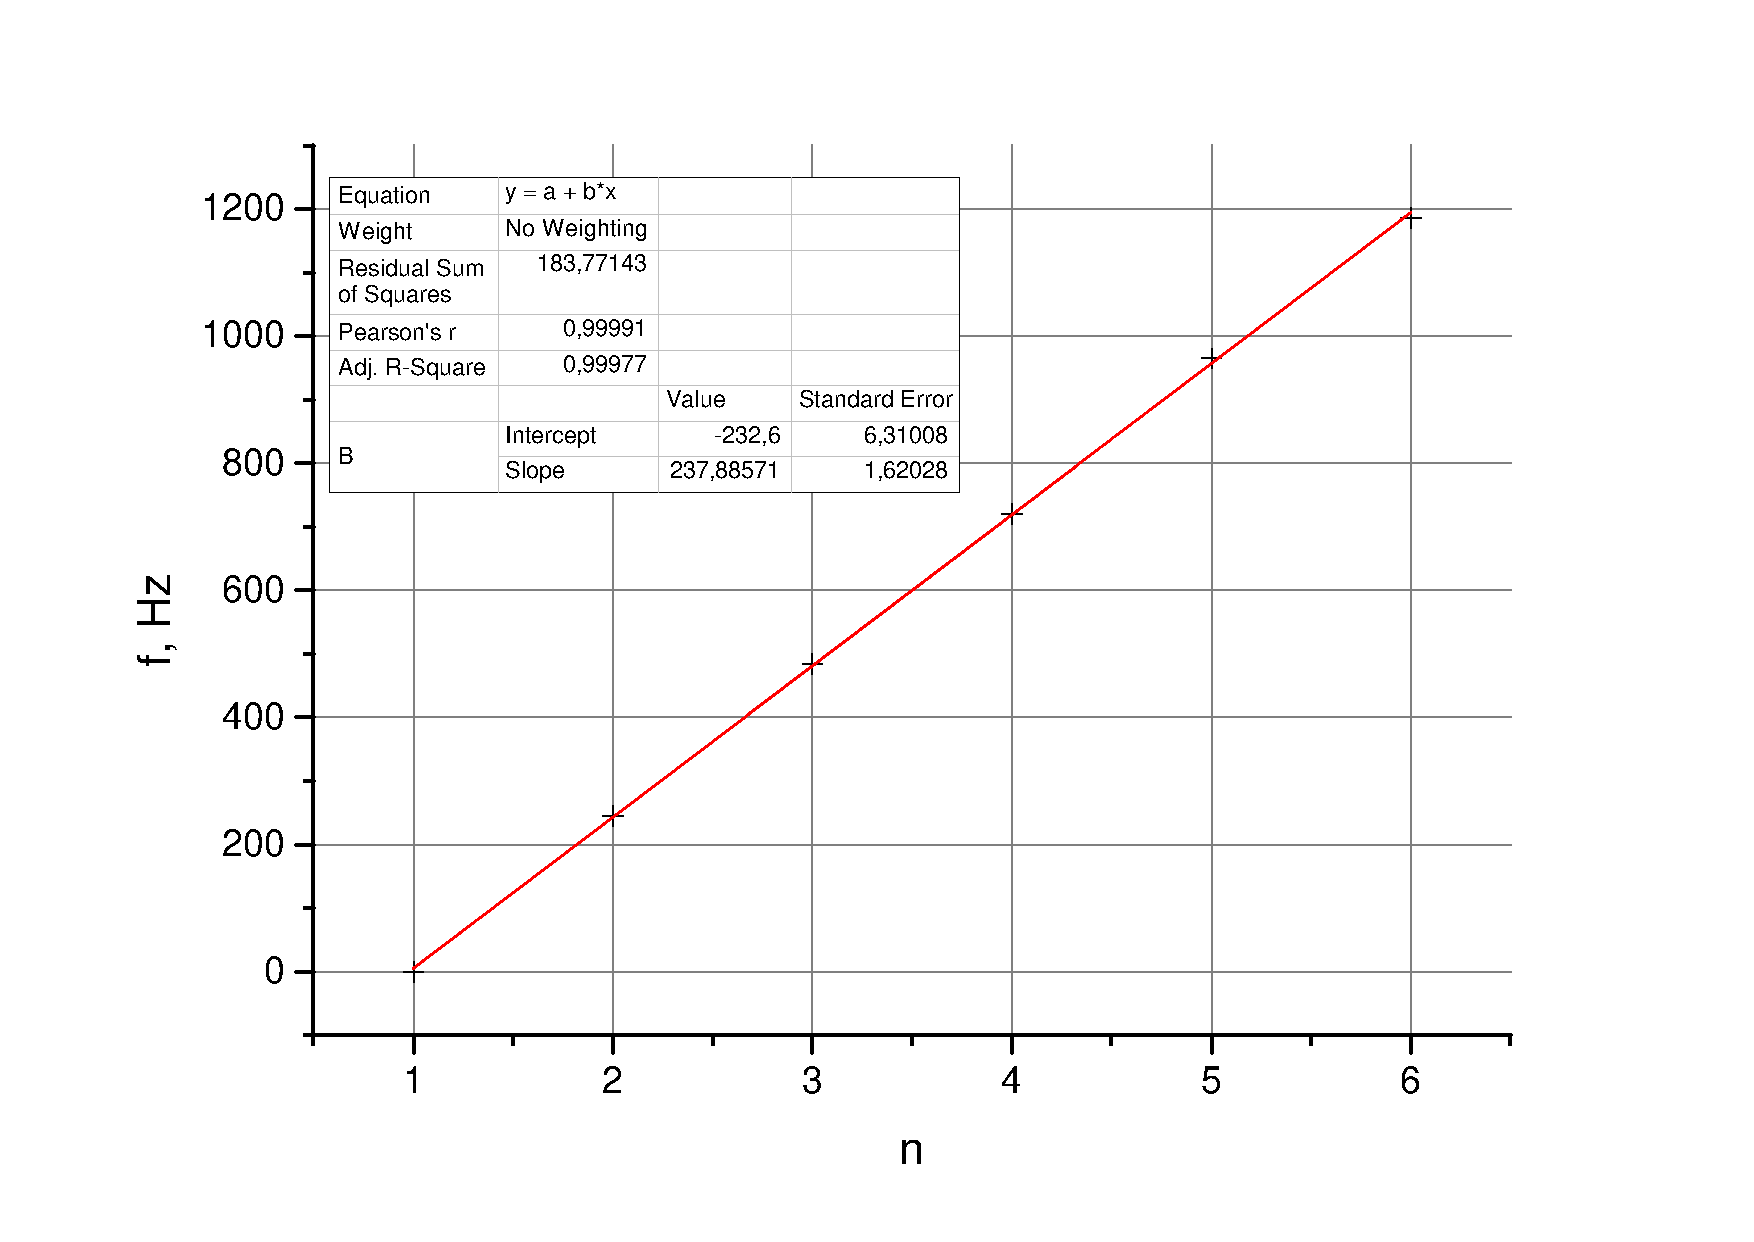
\includegraphics[width = 0.9\linewidth]{Graph5gr}
		
		\begin{center}
			\begin{tabular}{l | l | l | l | l | l}
				T, K & $\frac{c}{2L}$ & $\sigma\frac{c}{2L}$ & c, м/с & $\gamma$ & $\sigma\gamma\cdot 10^{-2}$\\ \hline
				23.6 & 232.05 & 2.32 & 343.43 & 1.34 & 1.99\\ \hline
				30.1 & 233.22 & 0.58 & 345.17 & 1.32 & 0.66  \\ \hline
				40 & 235.96 & 0.82 & 349.22 & 1.31 & 0.74  \\ \hline
				50 & 240.71 & 0.48 & 356.25 & 1.32 & 0.49  \\ \hline
				59 & 237.68 & 1.62 & 351.77 & 1.25 & 1.23  \\ \hline
			\end{tabular}
		\end{center}
		\subsection{Измерения на подвижной трубе}
		Измерим скорость звука в углекислом газе.
		\begin{center}
			\begin{tabular}{ l | l | l | l | l | l | l | l | l | l | l | l }
				\multicolumn{2}{|c}{$f=1468$ Гц} & \multicolumn{2}{|c}{$f=2355$ Гц} & \multicolumn{2}{|c}{$f=2432$ Гц} & \multicolumn{2}{|c}{$f=3325$ Гц}& \multicolumn{2}{|c}{$f=3822$ Гц}& \multicolumn{2}{|c}{$f=4984$ Гц}\\ \hline
				n & $L$, мм & n & $L$, мм & n & $L$, мм & n & $L$, мм & n & $L$, мм & n & $L$, мм \\ \hline
				1 & 700 & 1 & 723 & 1 & 700  & 1 & 704 & 1 & 723 & 1 & 701  \\ \hline
				2 & 715 & 2 & 716.6 & 2 & 706.7 & 2 & 708.2 & 2 & 719.7 & 2 & 704  \\ \hline
				3 & 721 & 3 & 710.2 & 3 & 712.8 & 3 & 712.5 & 3 & 716 & 3 & 706.9  \\ \hline
				  &     & 4 & 703.8 & 4 & 719.3 & 4 & 716.8 & 4 & 712.3 & 4 & 709.3  \\ \hline
				  &     &   &       &   &       & 5 & 721.2 & 5 & 708.6 & 5 & 712.2 \\ \hline
			      &     &   &       &   &       &   &       & 6 & 705 & 6 & 714.7   \\ \hline
			      &     &   &       &   &       &   &       & 7  & 701.3 & 7 & 718.2   \\ \hline
				  &     &   &       &   &       &   &       &    &       & 8 & 721   \\ \hline
			\end{tabular}
		\end{center}
		
		
		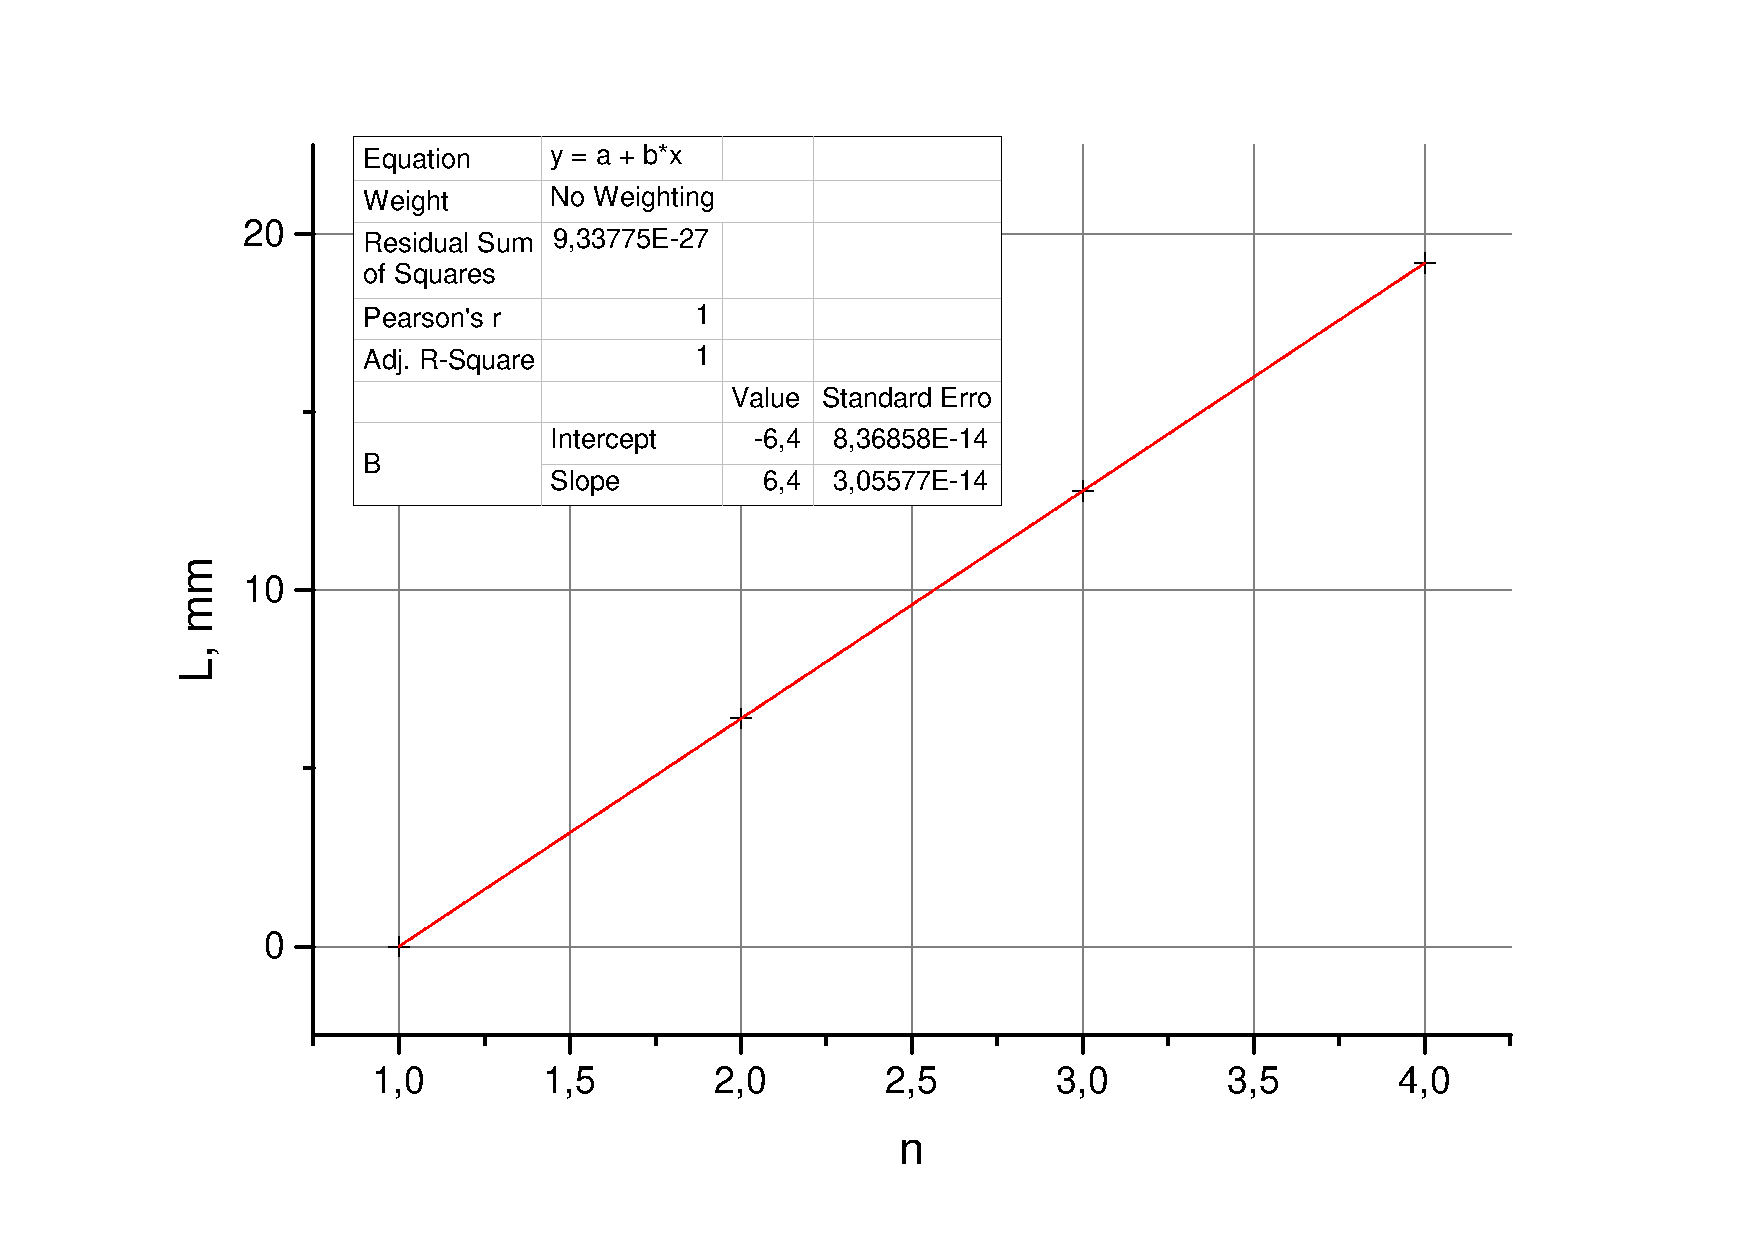
\includegraphics[width = 0.9\linewidth]{Graph1co2}
		
		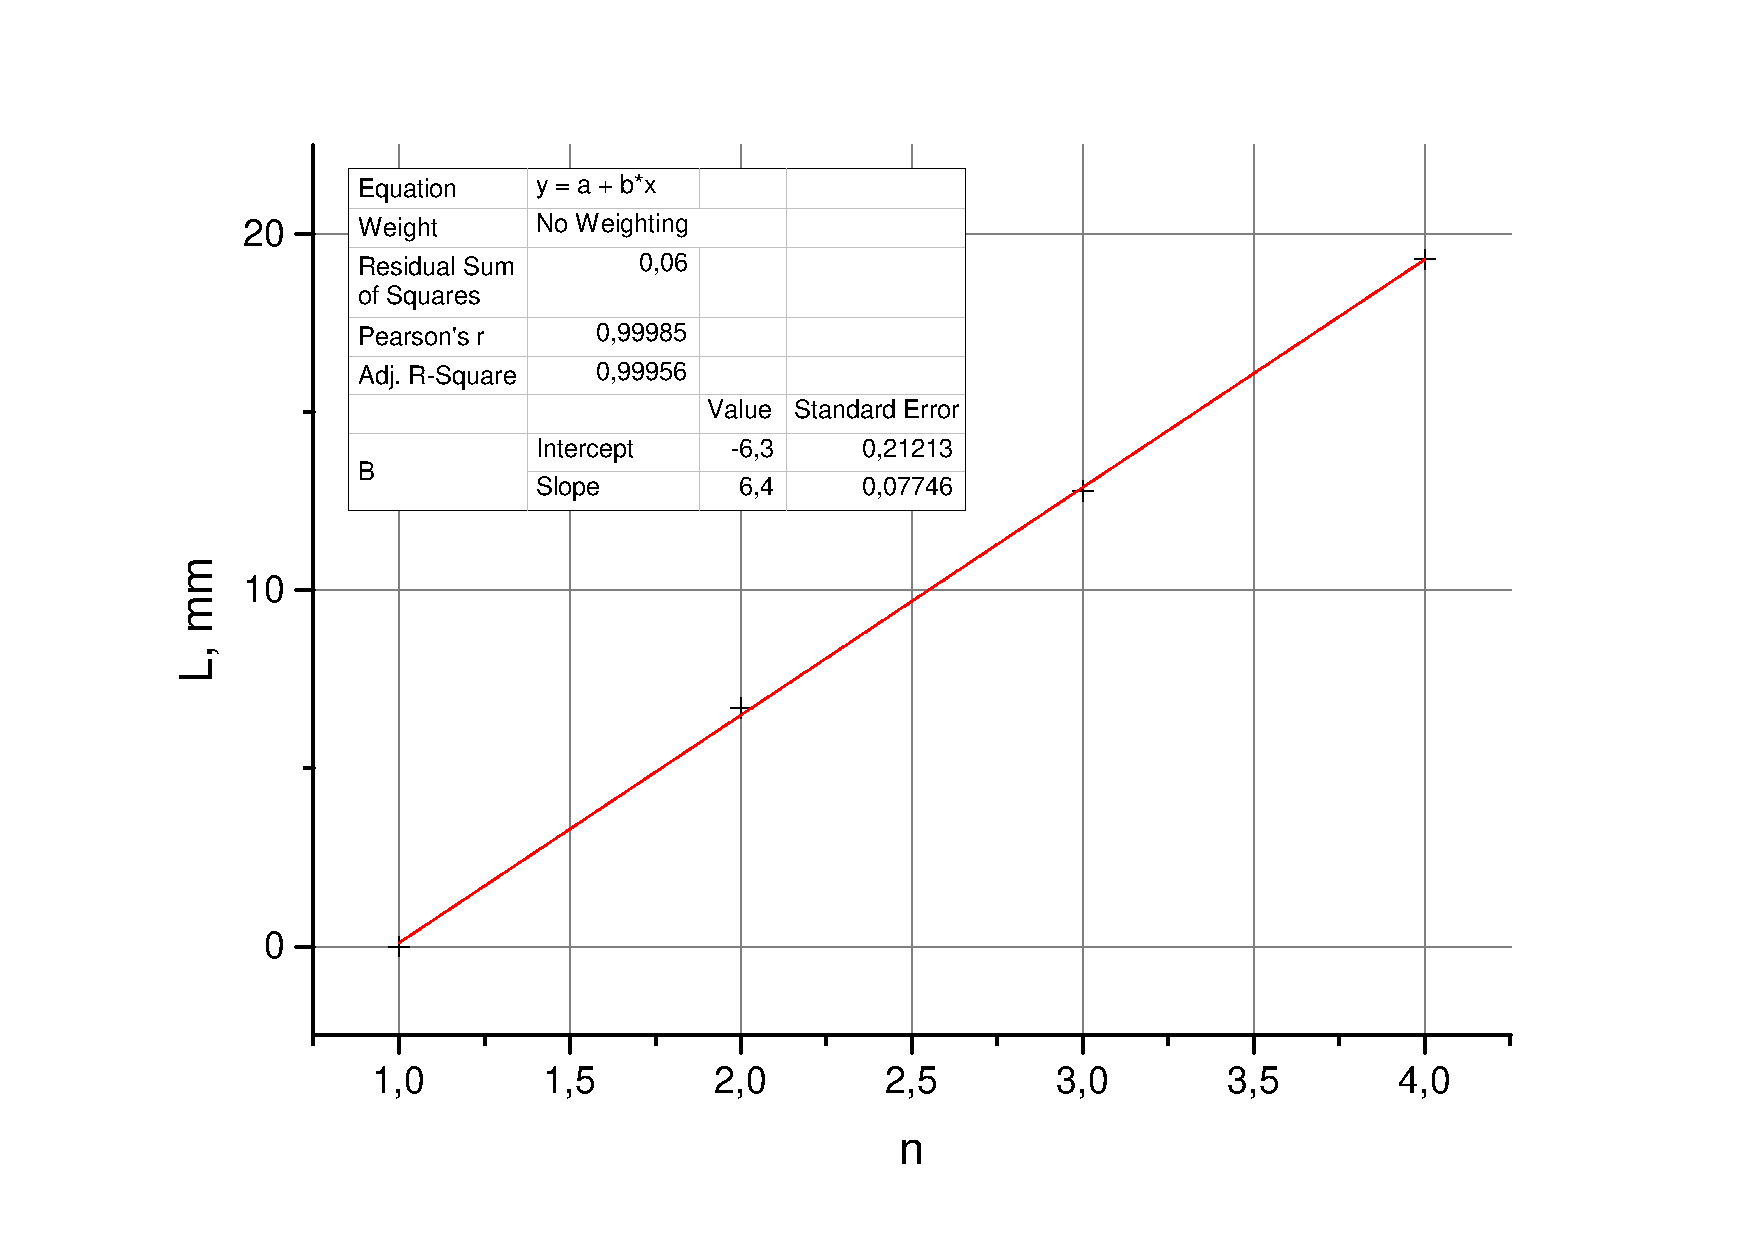
\includegraphics[width = 0.9\linewidth]{Graph2co2}
		
		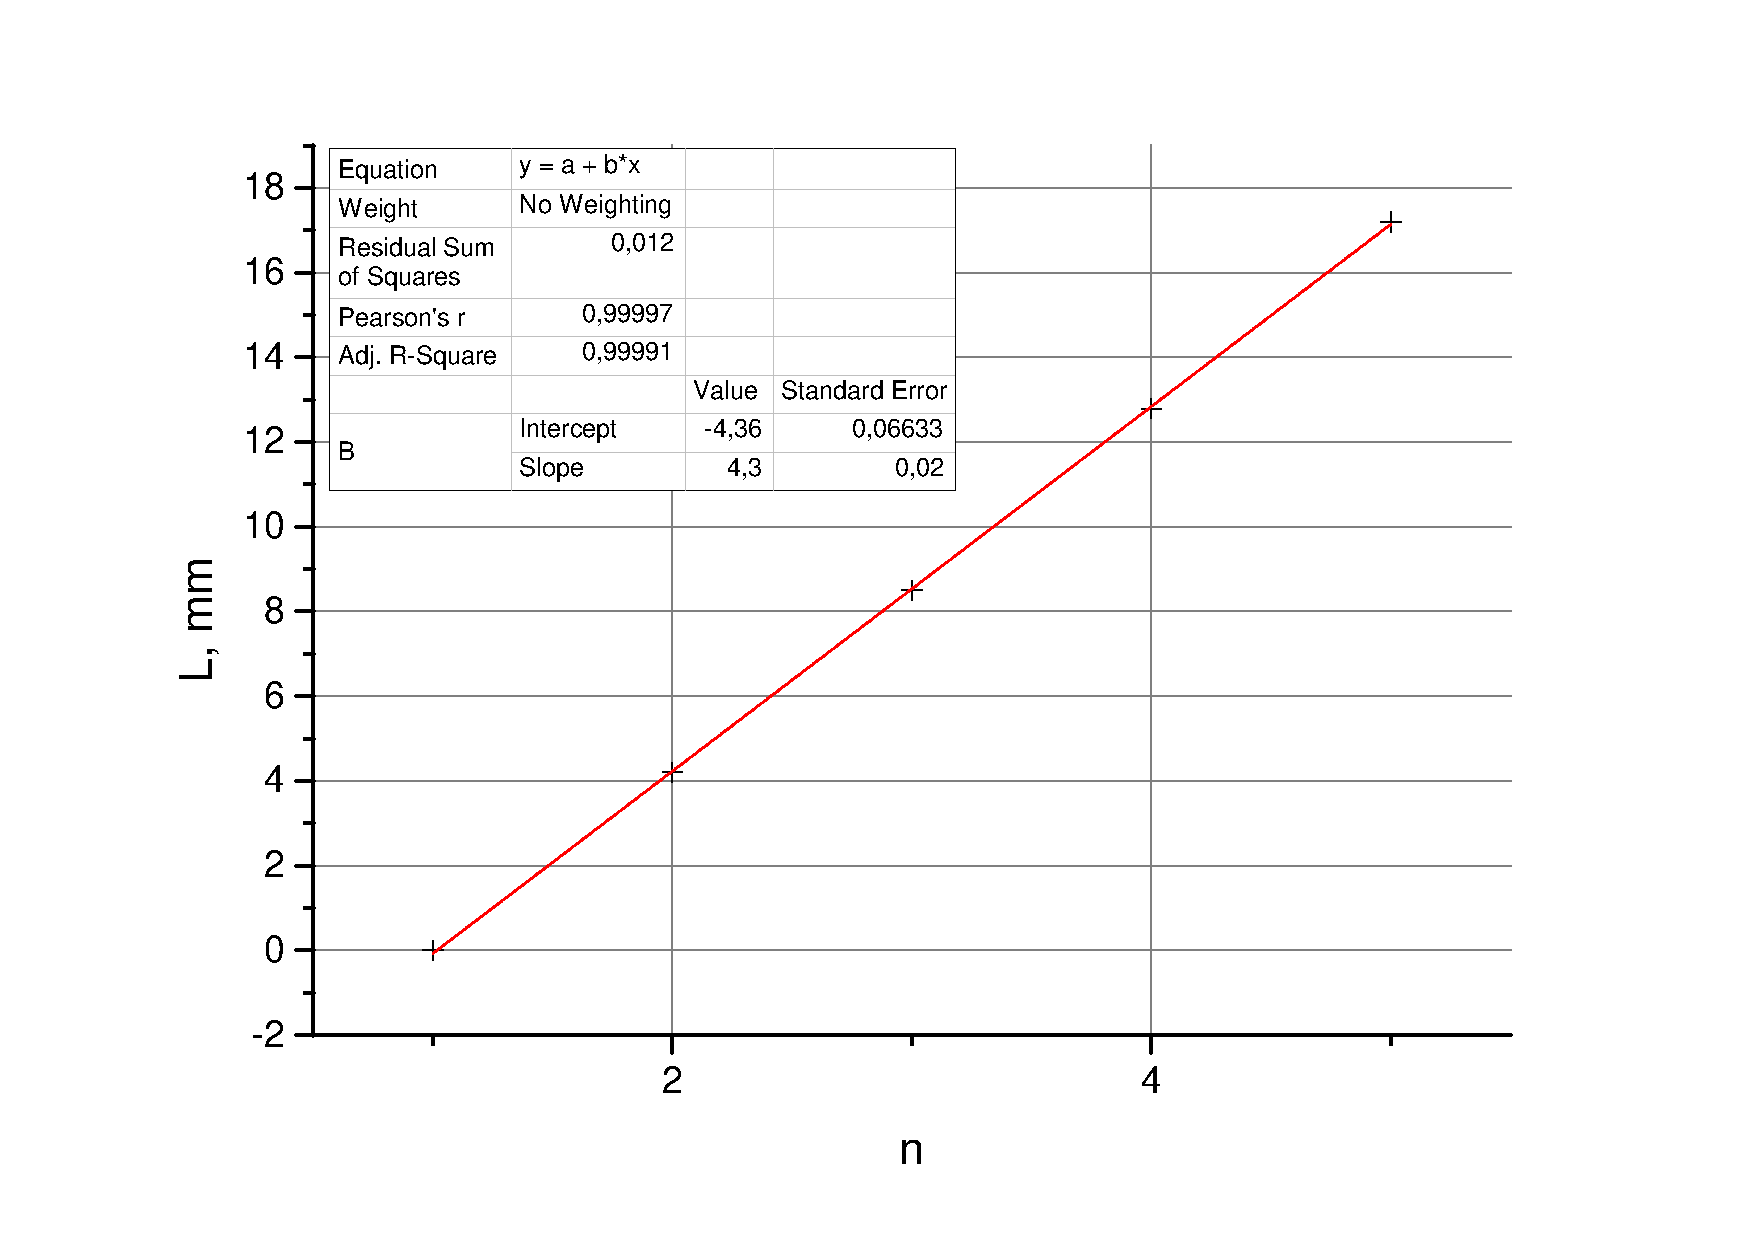
\includegraphics[width = 0.9\linewidth]{Graph3co2}
		
		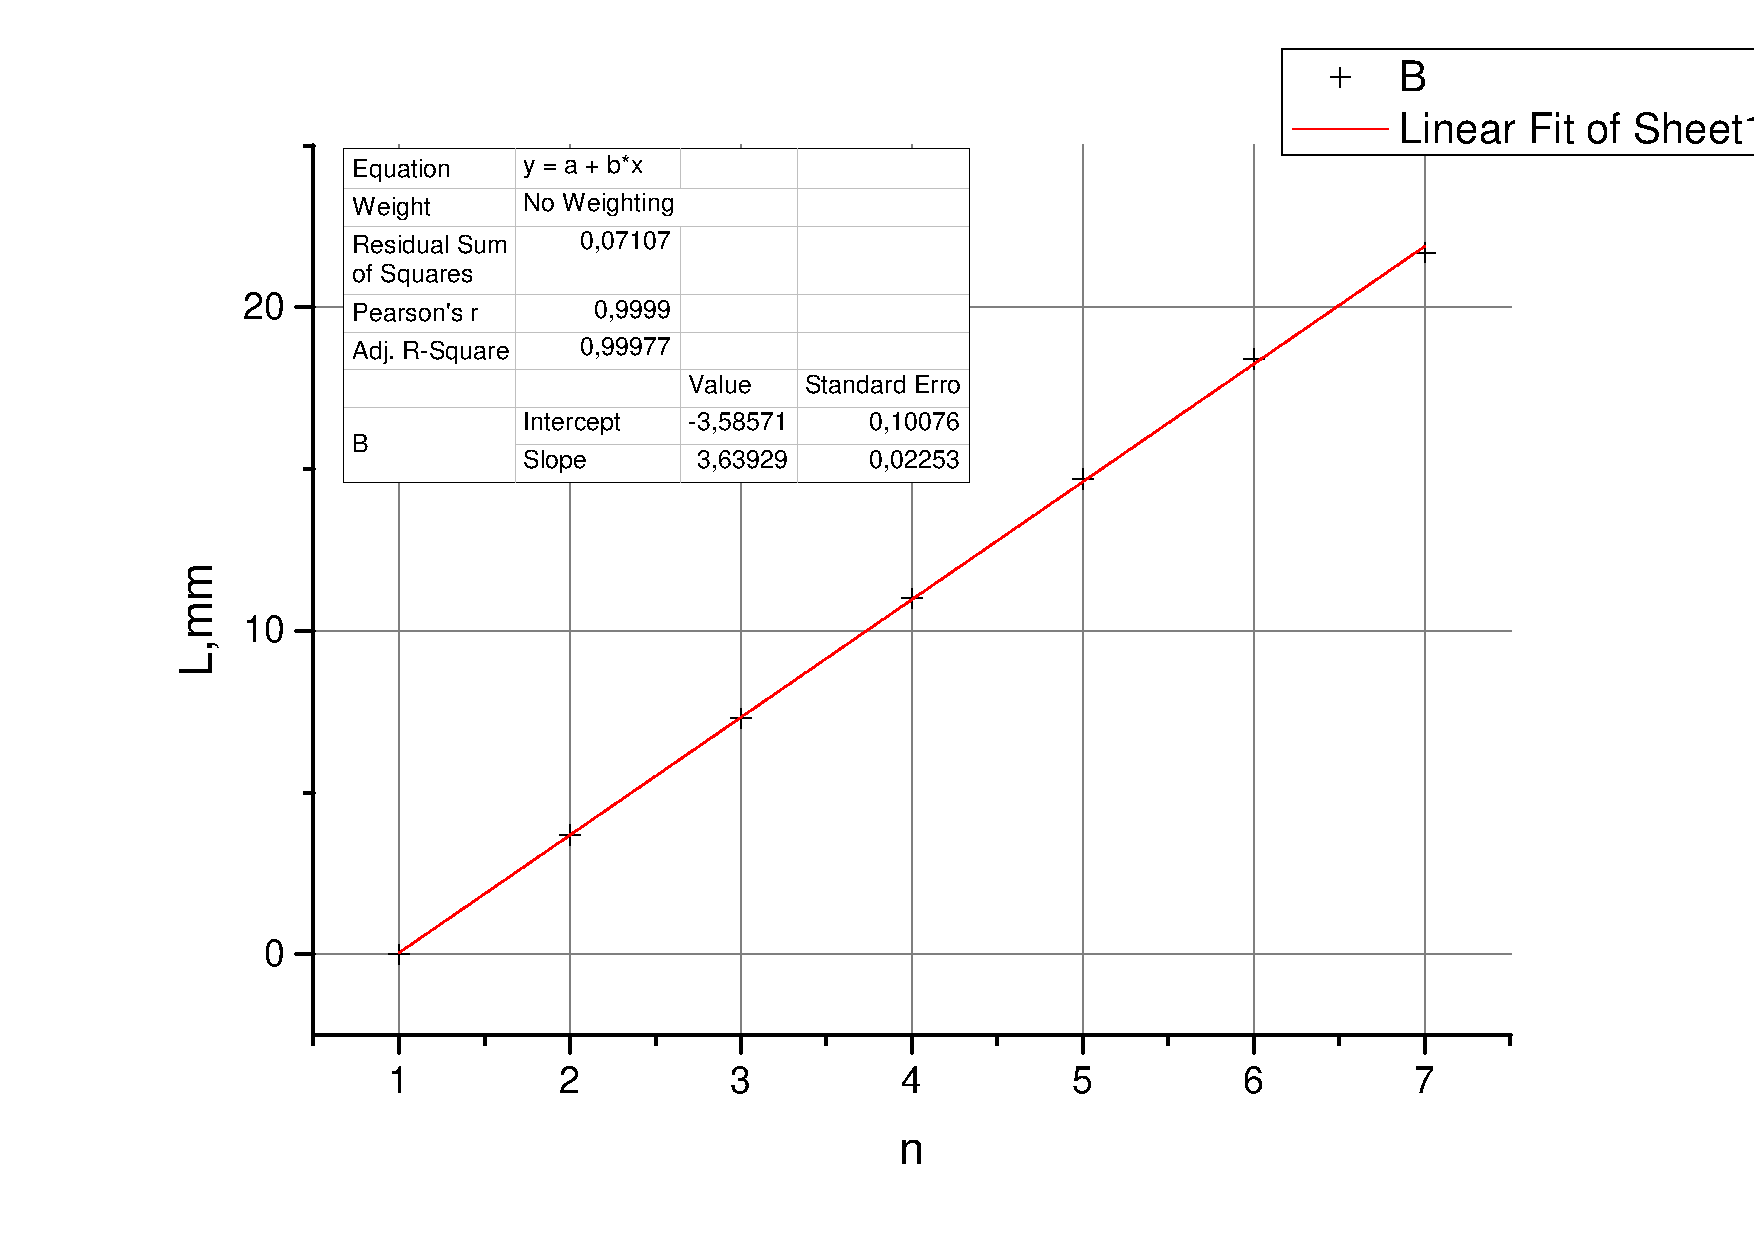
\includegraphics[width = 0.9\linewidth]{Graph4co2}
		
		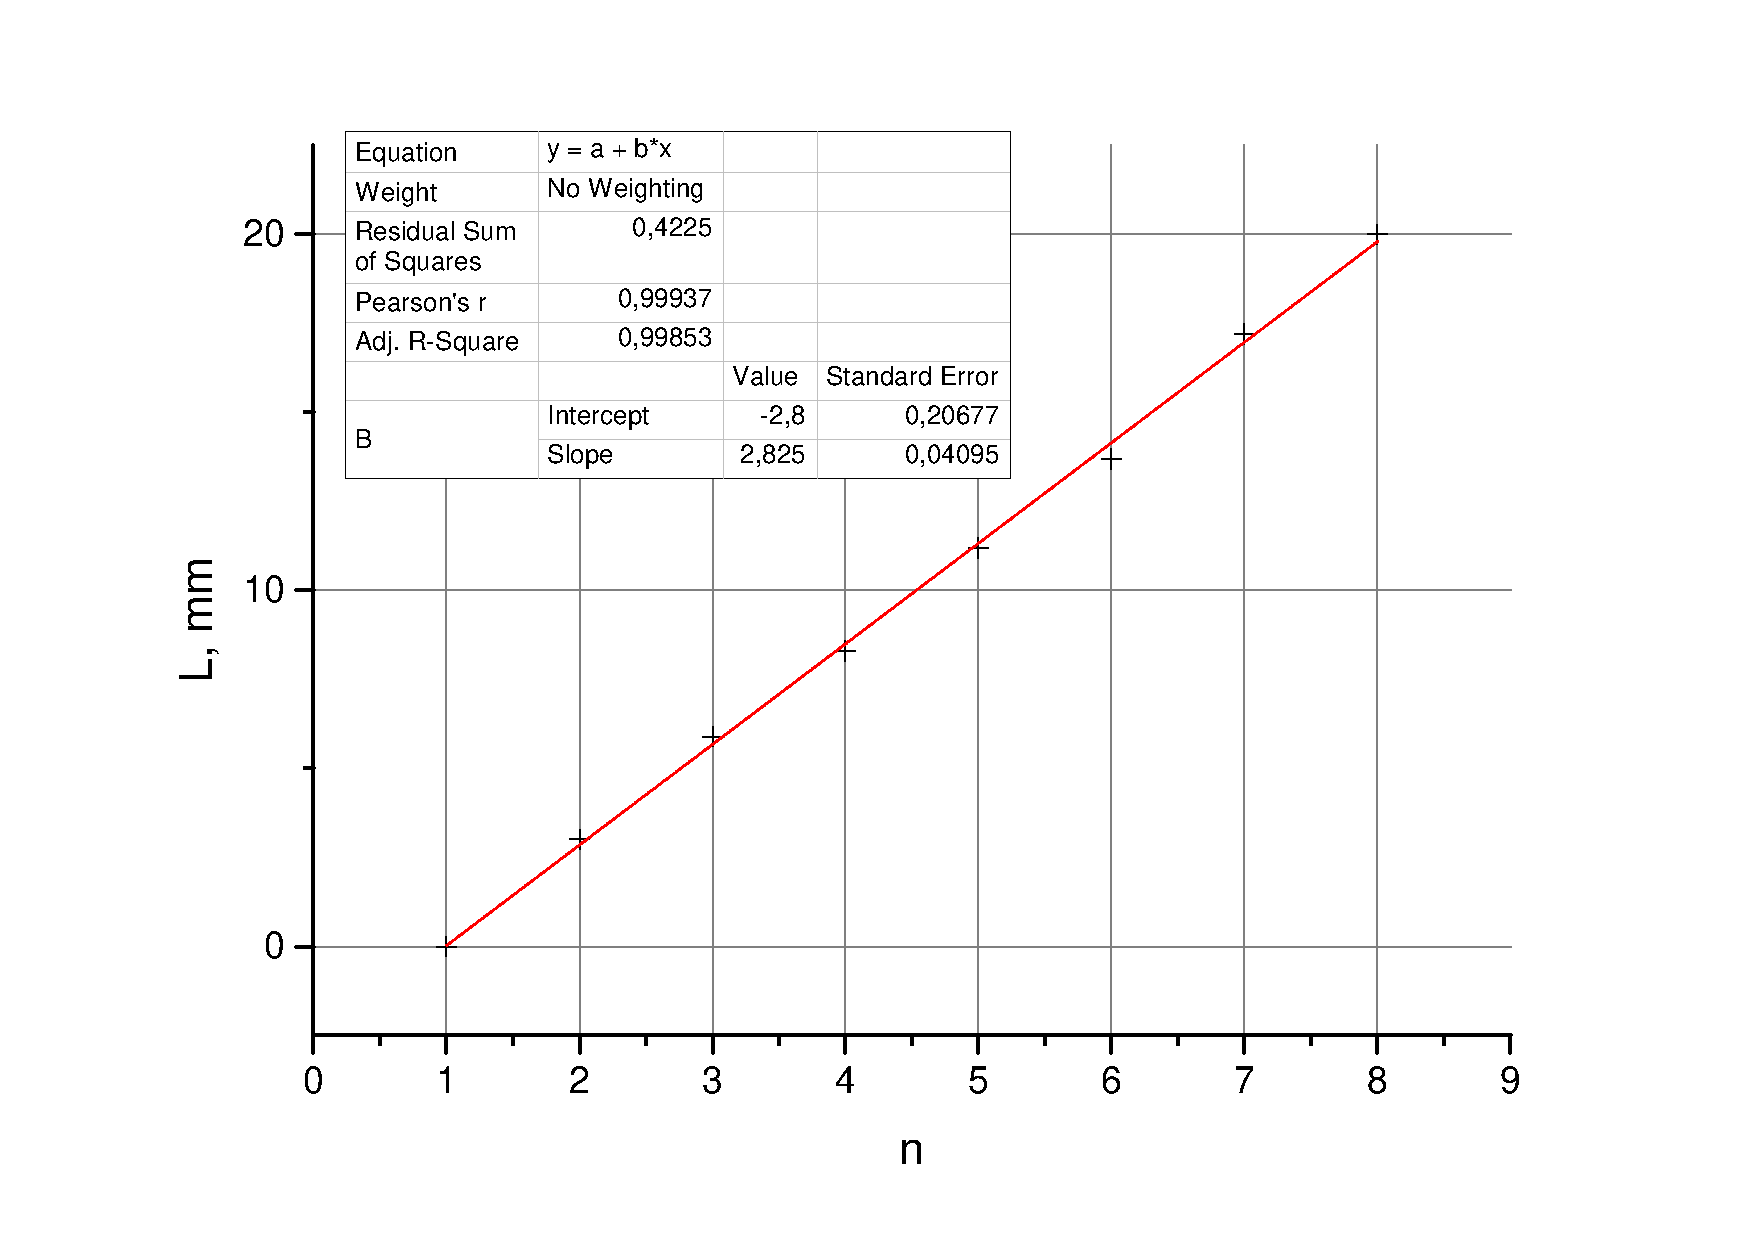
\includegraphics[width = 0.9\linewidth]{Graph5co2}
		
		\begin{center}
			\begin{tabular}{l | l | l | l | l | l | l}
				$f$, Гц & $\frac{\lambda}{2}\cdot 10^{-3}$, м & $\sigma\frac{\lambda}{2}\cdot 10^{-3}$ & c, м/с &$\sigma c$ & $\gamma$ & $\sigma\gamma$\\ \hline
				2355 & 6.4 & 0.21 & 301.4 & 6 & 1.62 & 0.05 \\ \hline
				2432 & 6.4 & 0.21 & 311.3 & 6.22 & 1.72 & 0.05\\ \hline
				3325 & 4.3 & 0.14 & 286 & 5.72 & 1.45 &  0.04 \\ \hline
				3822 & 3.6 & 0.12 & 275.1 & 5.5 & 1.34 &  0.04 \\ \hline
				4984 & 2.8 & 0.09 & 279.1 & 5.58 & 1.38 & 0.04  \\ \hline
			\end{tabular}
		\end{center}
		\newpage
		Измерим скорость звука в воздухе.
		\begin{center}
			\begin{tabular}{ l | l | l | l | l | l | l | l | l | l | l | l }
				\multicolumn{2}{|c}{$f=1748$ Гц} & \multicolumn{2}{|c}{$f=1845$ Гц} & \multicolumn{2}{|c}{$f=2200$ Гц} & \multicolumn{2}{|c}{$f=2546$ Гц}& \multicolumn{2}{|c}{$f=2873$ Гц}& \multicolumn{2}{|c}{$f=2891$ Гц}\\ \hline
				n & $L$, мм & n & $L$, мм & n & $L$, мм & n & $L$, мм & n & $L$, мм & n & $L$, мм \\ \hline
				1 & 700   & 1 & 723 & 1 & 700  & 1 & 723 & 1 & 700 & 1 & 723  \\ \hline
				2 & 709.6 & 2 & 715.8 & 2 & 708.1 & 2 & 716.6 & 2 & 706.5 & 2 & 717.6  \\ \hline
				3 & 719.4 & 3 & 704.6 & 3 & 715.8 & 3 & 709.6 & 3 & 712.5 & 3 & 711.6  \\ \hline
				&         &   &       &   &       & 4 & 703   & 4 & 718.4 & 4 & 705.8  \\ \hline
				&         &   &       &   &       &   &       &   &       & 5 & 700 \\ \hline
			\end{tabular}
		\end{center}
				
				
	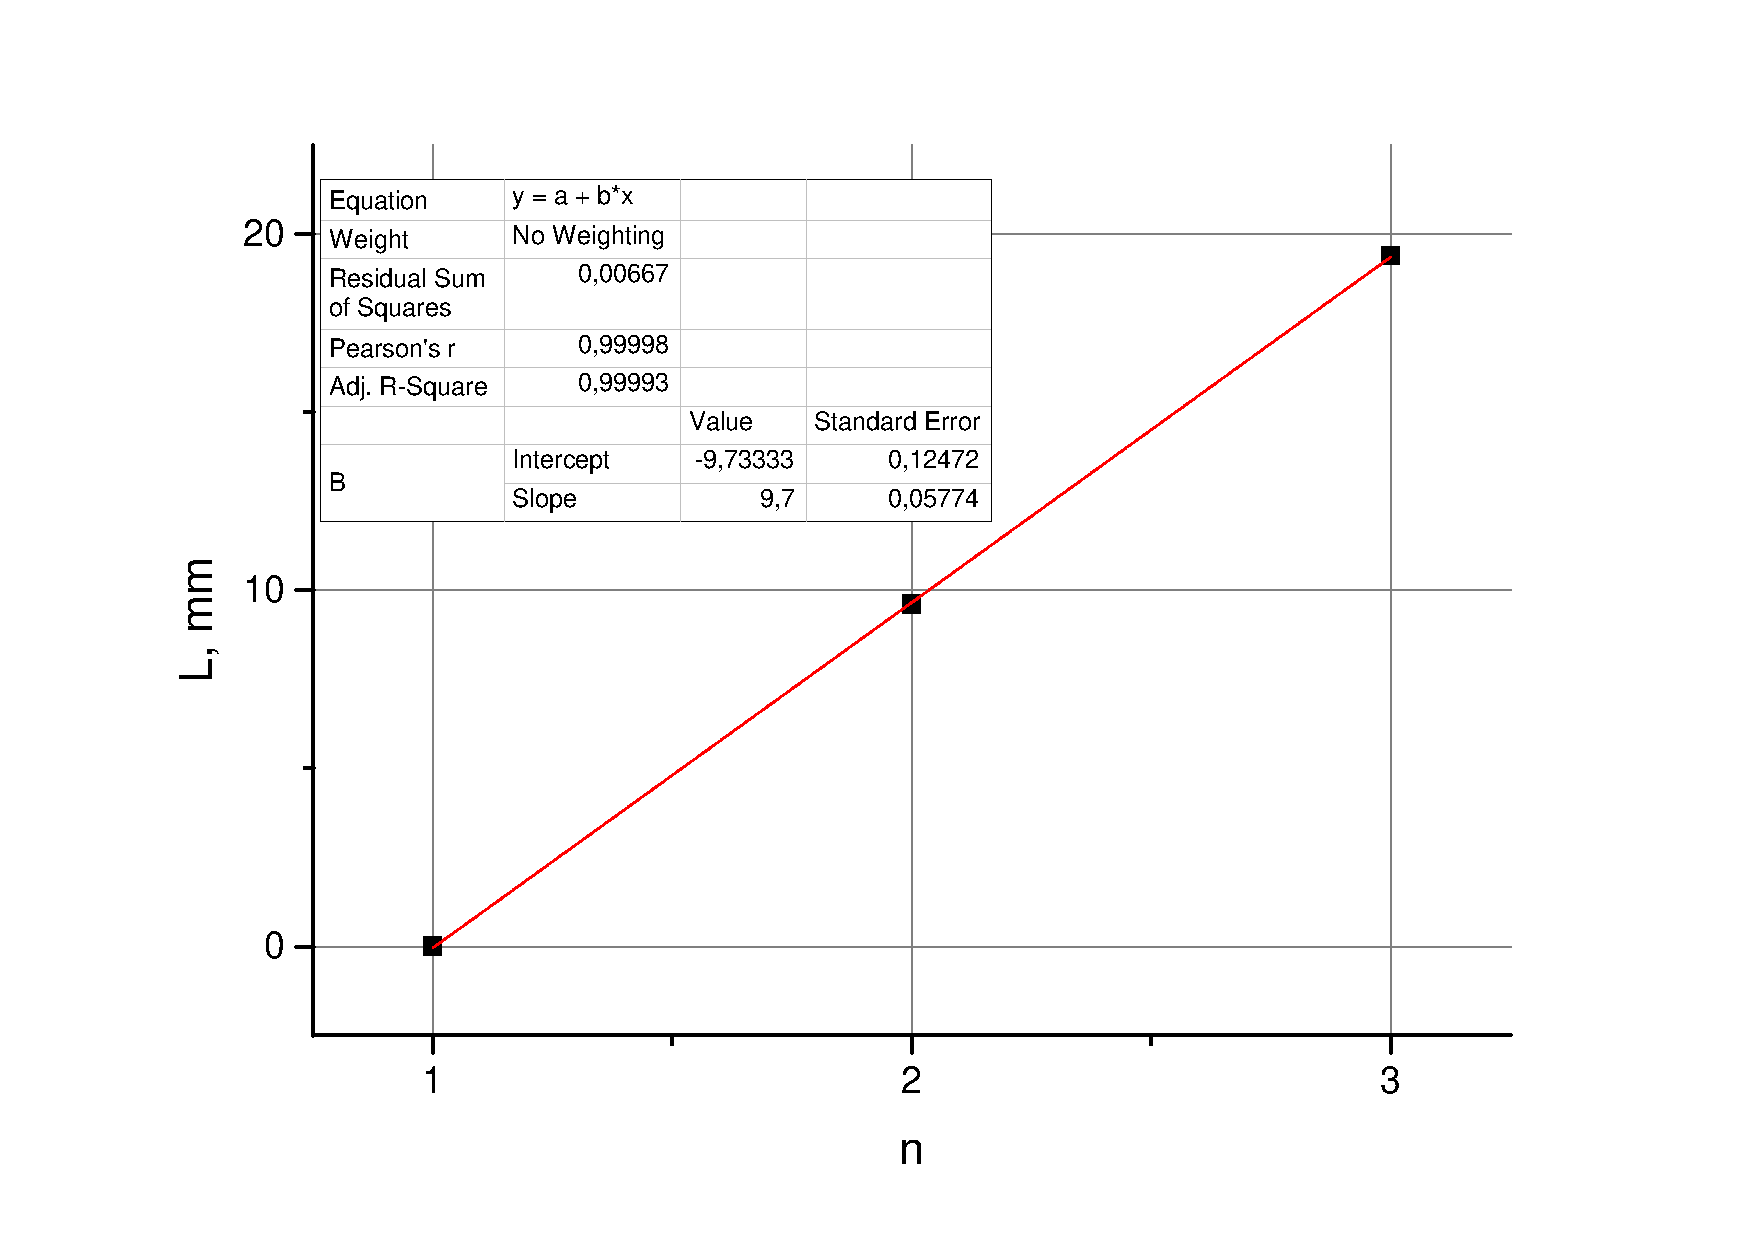
\includegraphics[width = 0.8\linewidth]{Graph1air}
				
	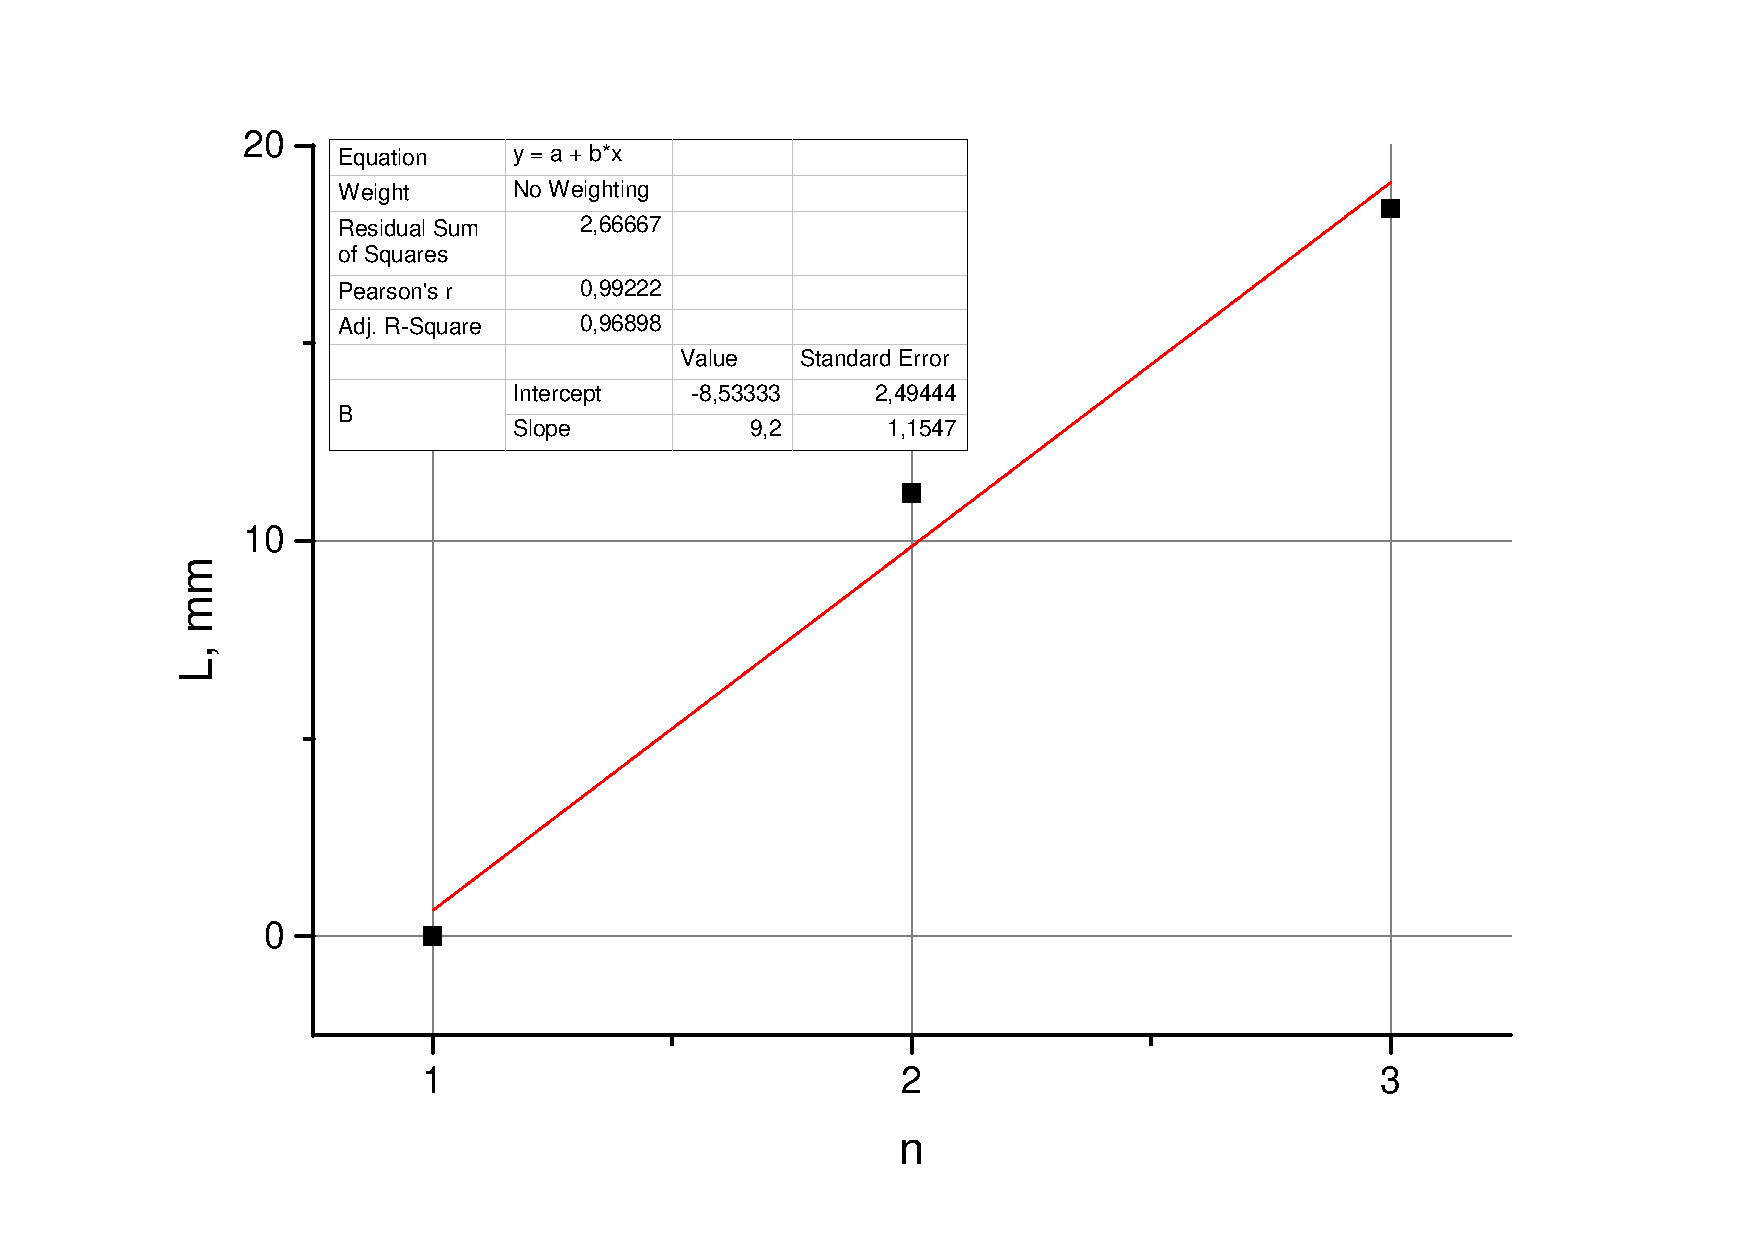
\includegraphics[width = 0.8\linewidth]{Graph2air}
				
	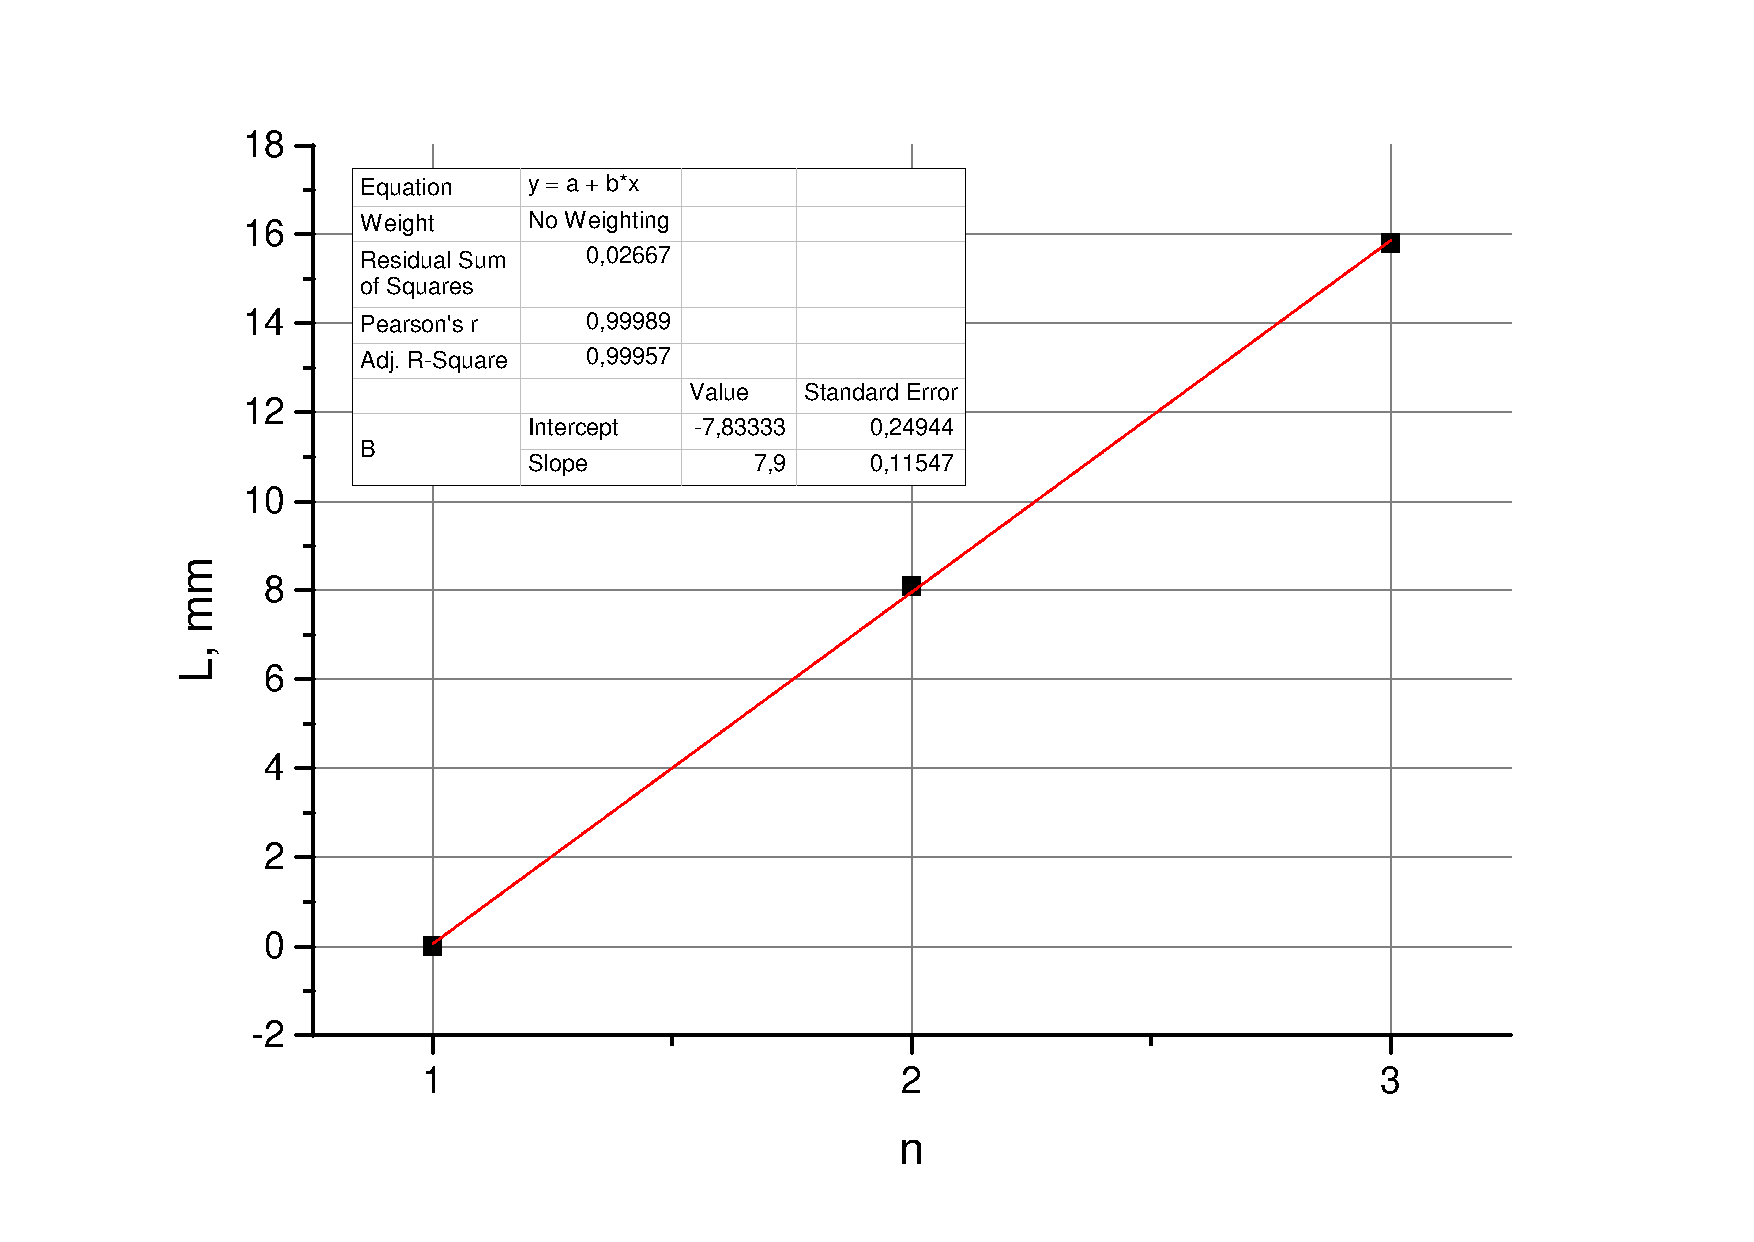
\includegraphics[width = 0.8\linewidth]{Graph3air}
				
	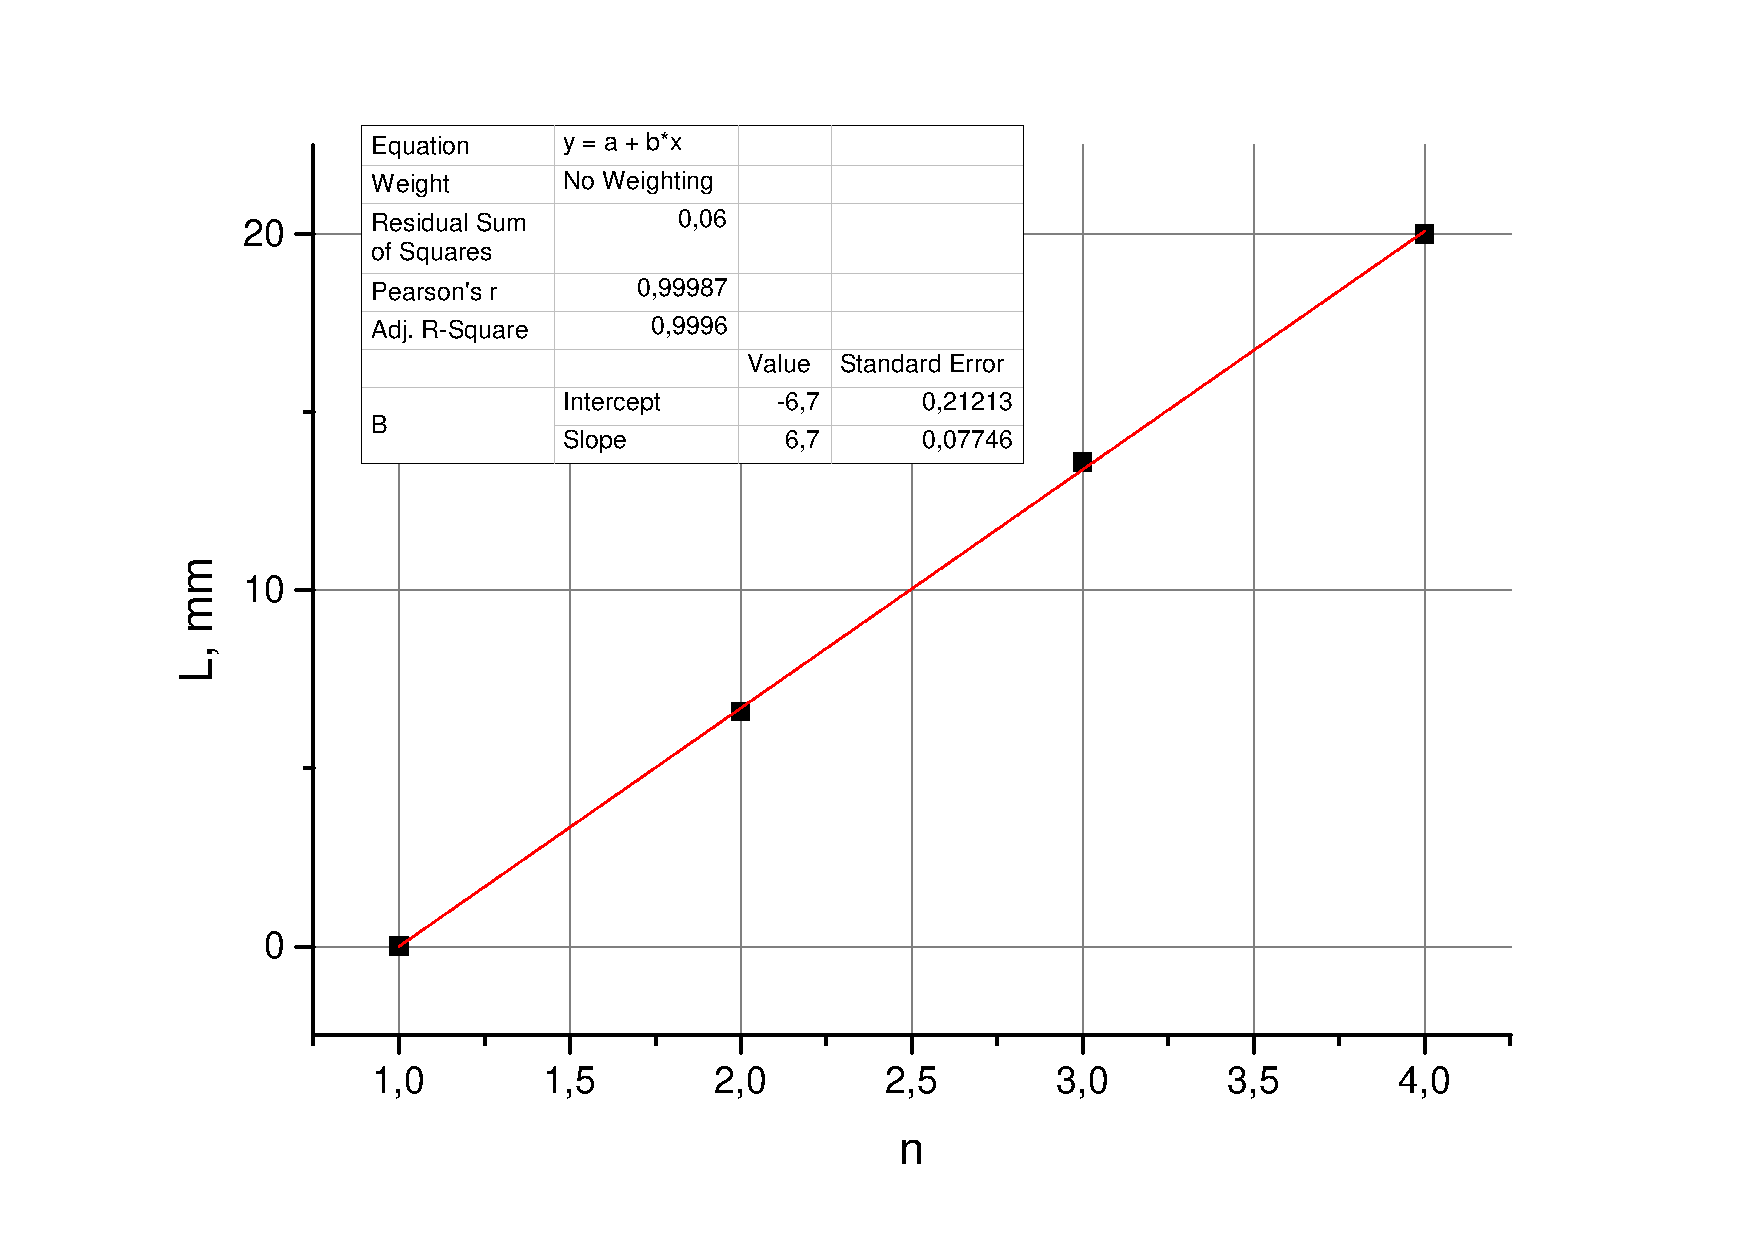
\includegraphics[width = 0.8\linewidth]{Graph4air}
				
	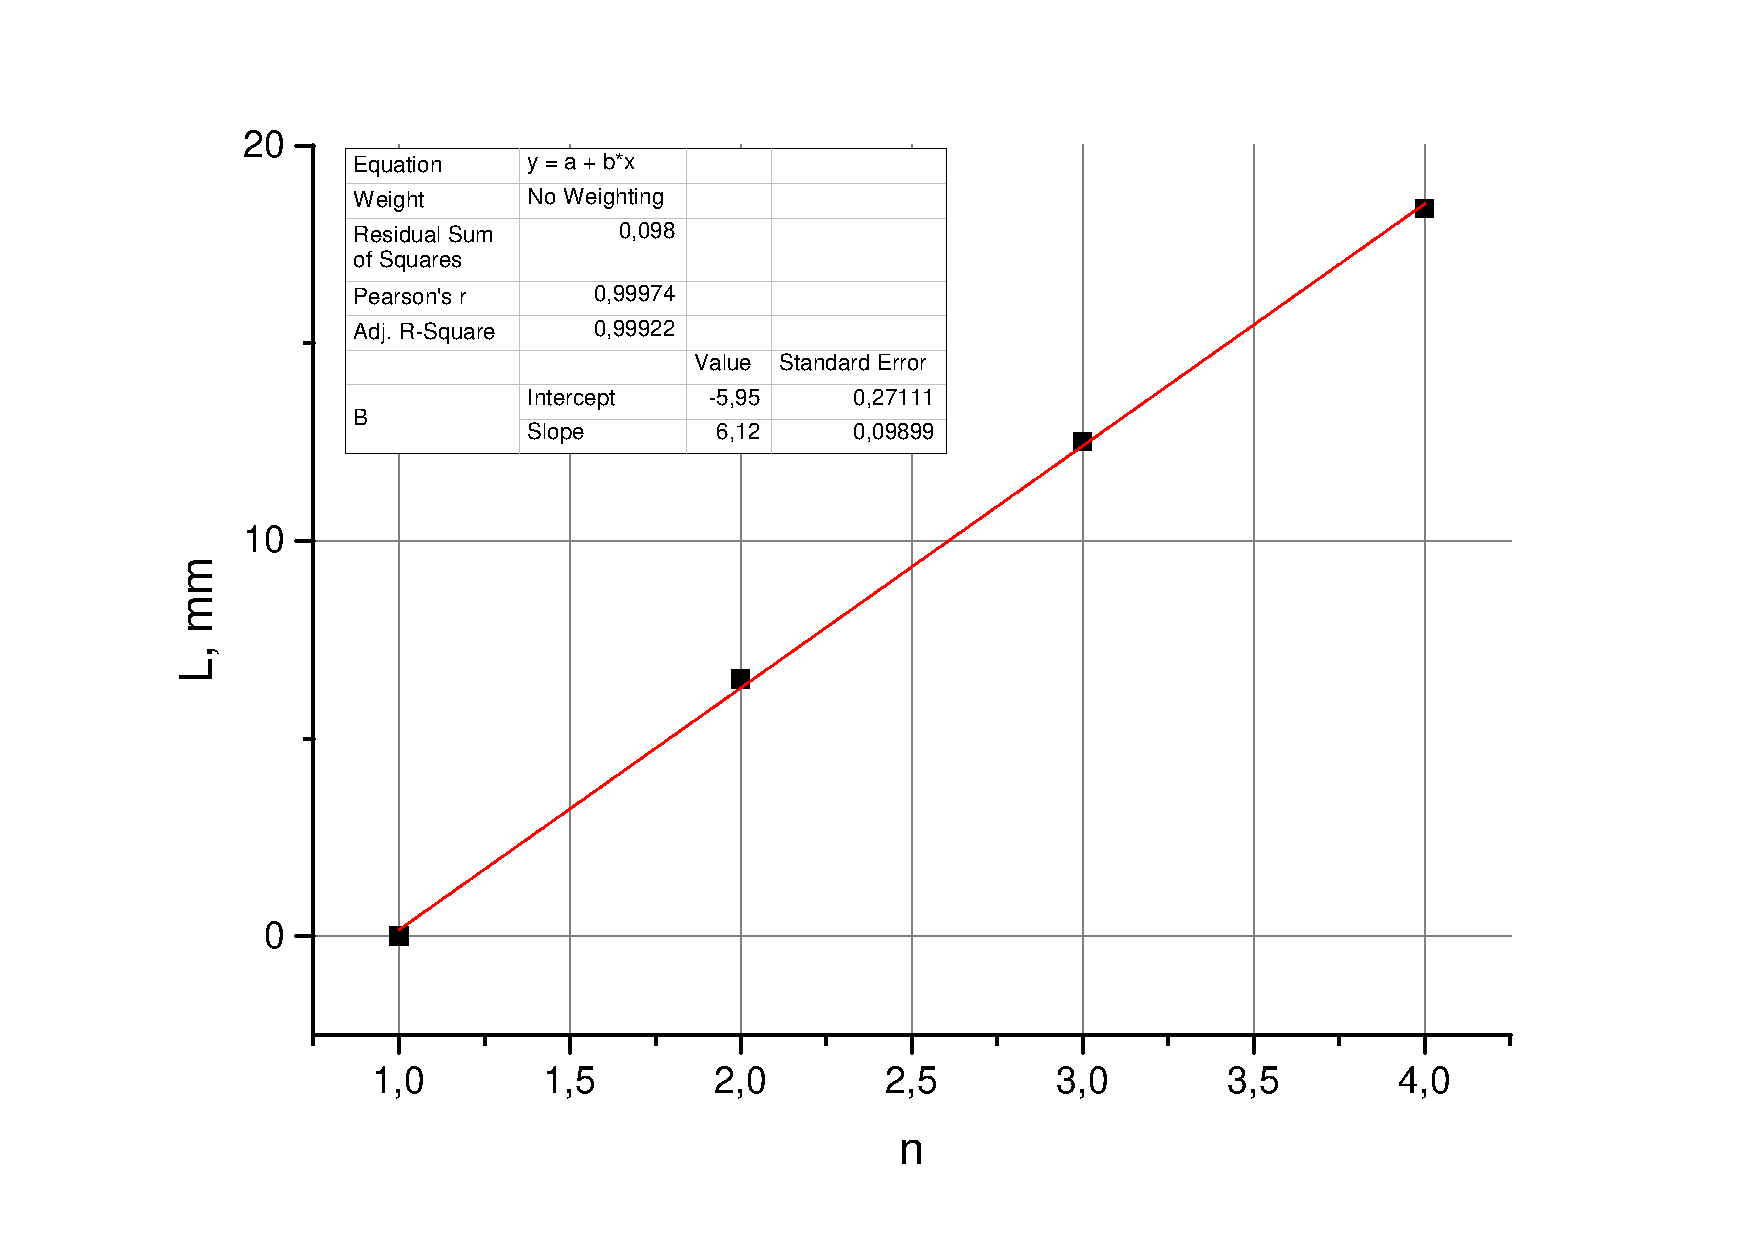
\includegraphics[width = 0.8\linewidth]{Graph5air}
		
		\begin{center}
			\begin{tabular}{l | l | l | l | l | l | l}
				$f$, Гц & $\frac{\lambda}{2}\cdot 10^{-3}$, м & $\sigma\frac{\lambda}{2}\cdot 10^{-3}$ & c, м/с &$\sigma c$ & $\gamma$ & $\sigma\gamma$\\ \hline
				1845 & 9.7 & 0.97 & 358 & 3.5 & 1.45 & 0.03 \\ \hline
				2200 & 9.2 & 0.92 & 404.8 & 4 & 1.85 & 0.04 \\ \hline
				2546 & 7.9 & 0.79 & 402.2 & 4 & 1.83 & 0.04\\ \hline
				2873 & 6.7 & 0.67 & 385 & 3.8 & 1.68 &  0.04 \\ \hline
				2891 & 6.12 & 0.61 & 353.8 & 3.5 & 1.41 &  0.03 \\ \hline
			\end{tabular}
		\end{center}	
	\section{Вывод}
		По измерению скорости звука в газе можно определить $\frac{C_p}{C_v}$ данного газа. По результатам измерений наиболее соответствующий реальности результат получился в неподвижной трубе. В раздвижной трубе наблюдаются значительные отклонения. Это может быть связано с тем, что измерения проводятся при приоткрытом газовом кране, и поступления газа в трубу превышают его утечки через соединения.
		
\end{document}


